 \section{Particle types}
 
 Particles can be identified by reconstructing their mass using the momentum measurement from the wire chamber track and the speed $\beta$ from the time of flight measurement:
 
 \begin{equation}\label{eq_beta}
 \beta = d / c t
 \end{equation}
 where $d$ is the distance between the two ToF arms providing a time of flight measurement $t$ in seconds. During period 2 the ToF arms were 13.1564 metres apart, whereas in period 3 this distance was shortened to 9.70772 metres. The speed of light $c$ is used to normalise the velocity.
 
 The mass is then
 
   \begin{equation}\label{eq_mass}                                                                                                                                                               
  m = p /(\gamma*c*\beta)
 \end{equation}
 where $\gamma$ is the Lorentz factor ($\frac{1}{\sqrt{1-\beta^2} }$) and $p$ is the momentum as measured using the wire chamber track curvature in the magnetic field.
 
 \begin{figure}[h]	
 \centering   
            \begin{subfigure}[b]{0.24\textwidth}
            \centering
            %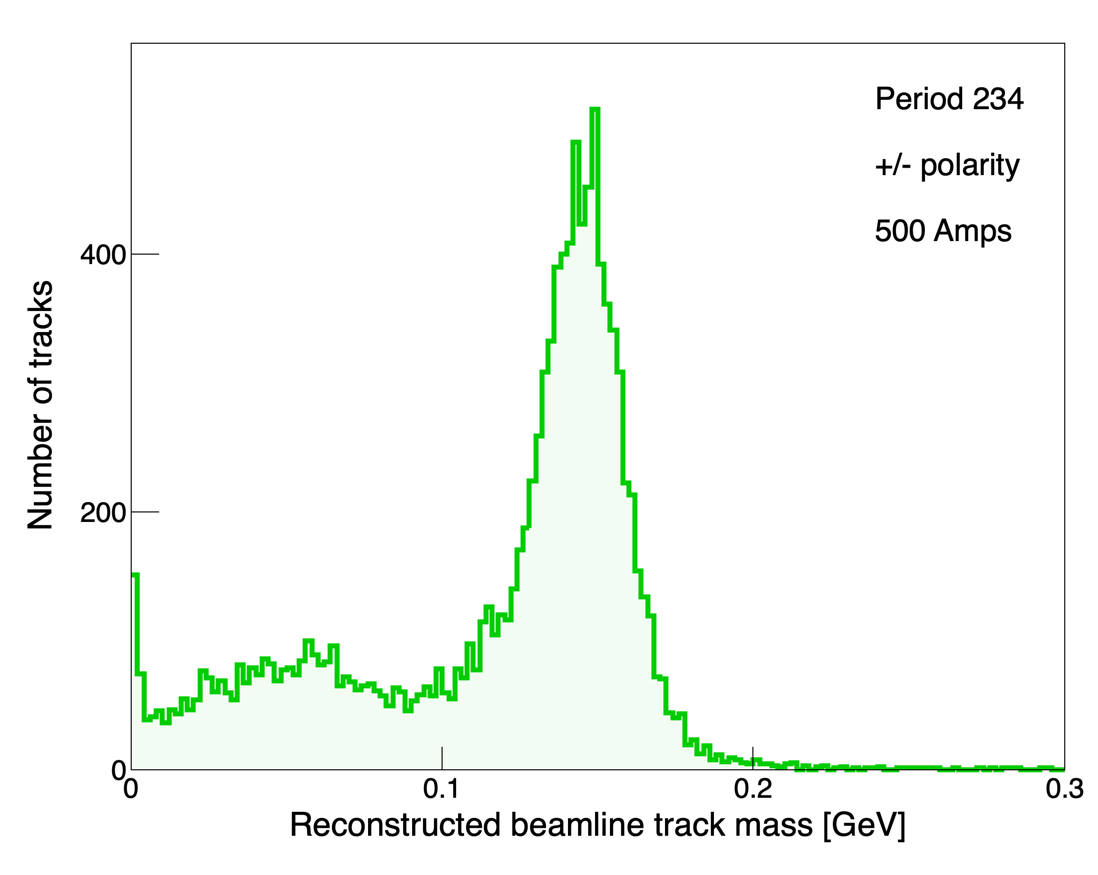
\includegraphics[width=\textwidth]{pimu-figsingle_period234_mass_level0_posneg_stats_500Amps.png} pimu_period234_mass_level4_posneg_stats_Mom1250.0_Cur1.png
            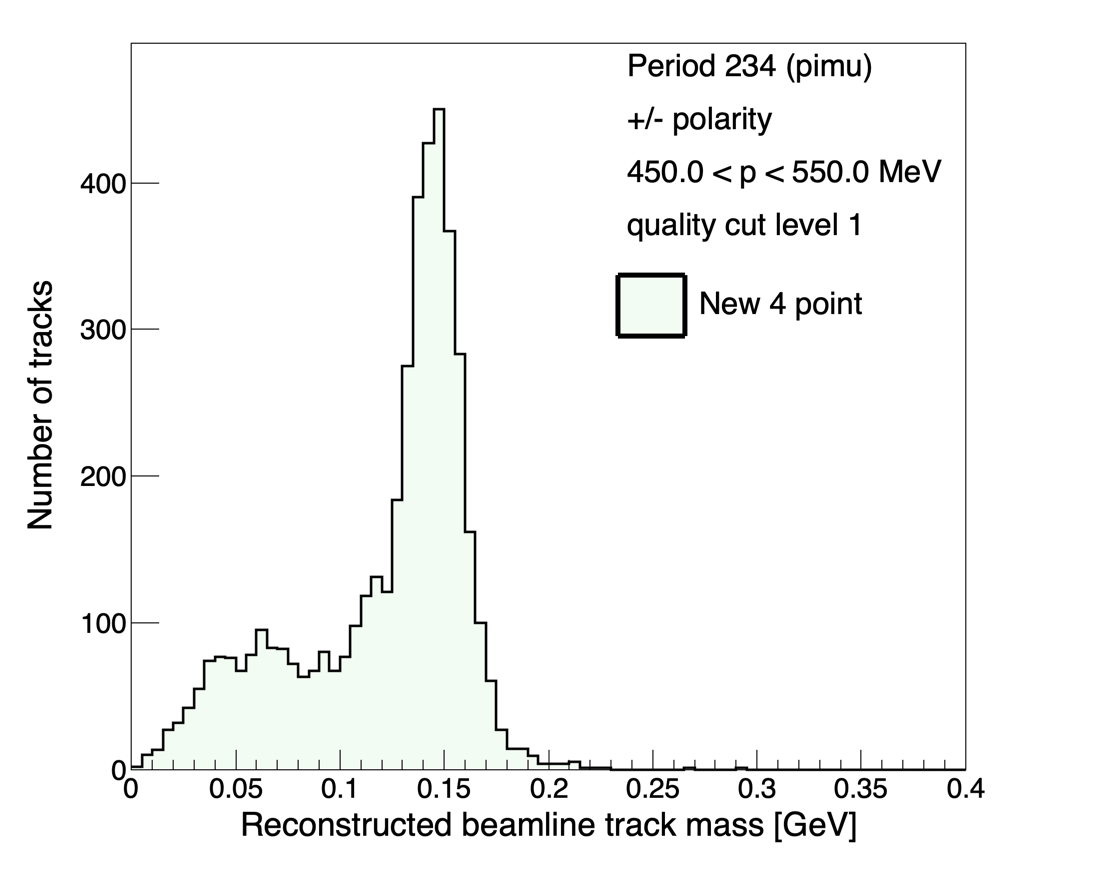
\includegraphics[width=\textwidth]{pimu_period234_mass_level0_posneg_stats_Mom500.0_Cur1.png}
            \caption{500 A}
            \label{fig_mpimu500}
            \end{subfigure}
             \hfill   
            \begin{subfigure}[b]{0.24\textwidth}
            \centering
            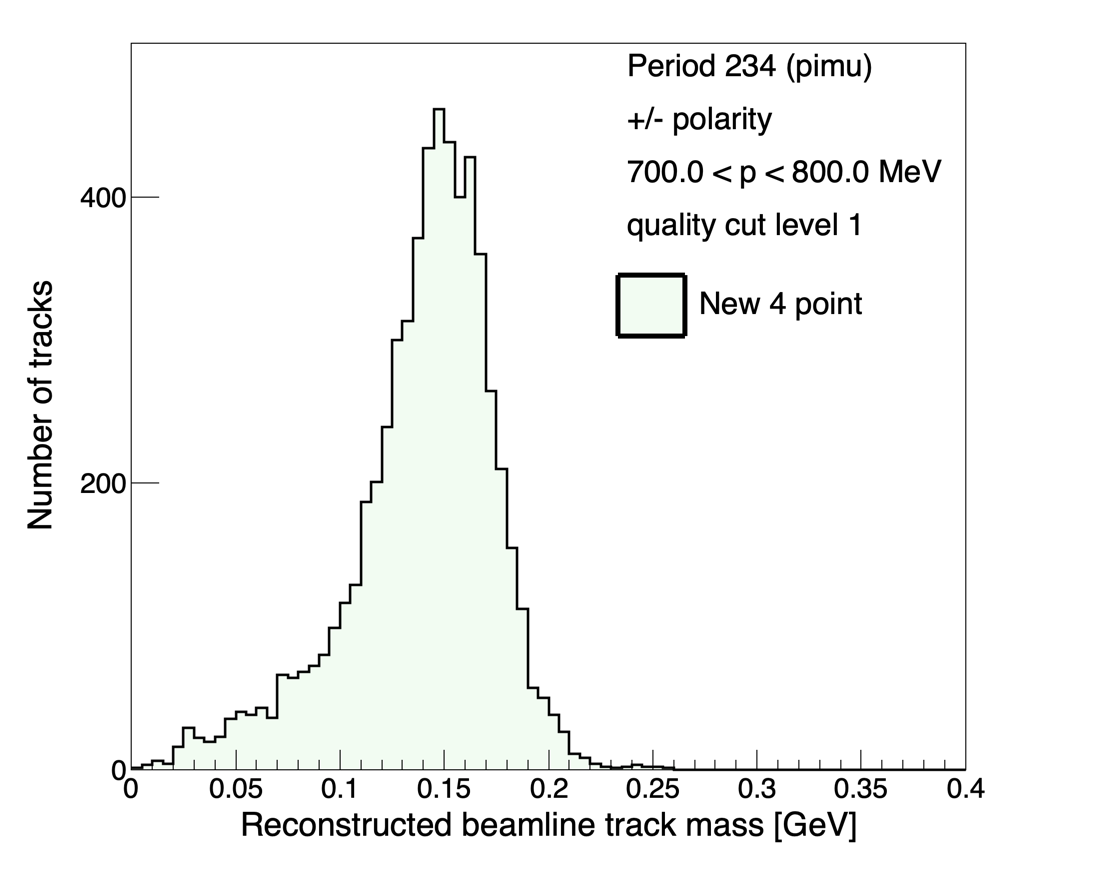
\includegraphics[width=\textwidth]{pimu_period234_mass_level0_posneg_stats_Mom750.0_Cur1.png}
            \caption{750 A}
            \label{fig_mpimu750}
            \end{subfigure}
             \hfill   
            \begin{subfigure}[b]{0.24\textwidth}
            \centering
            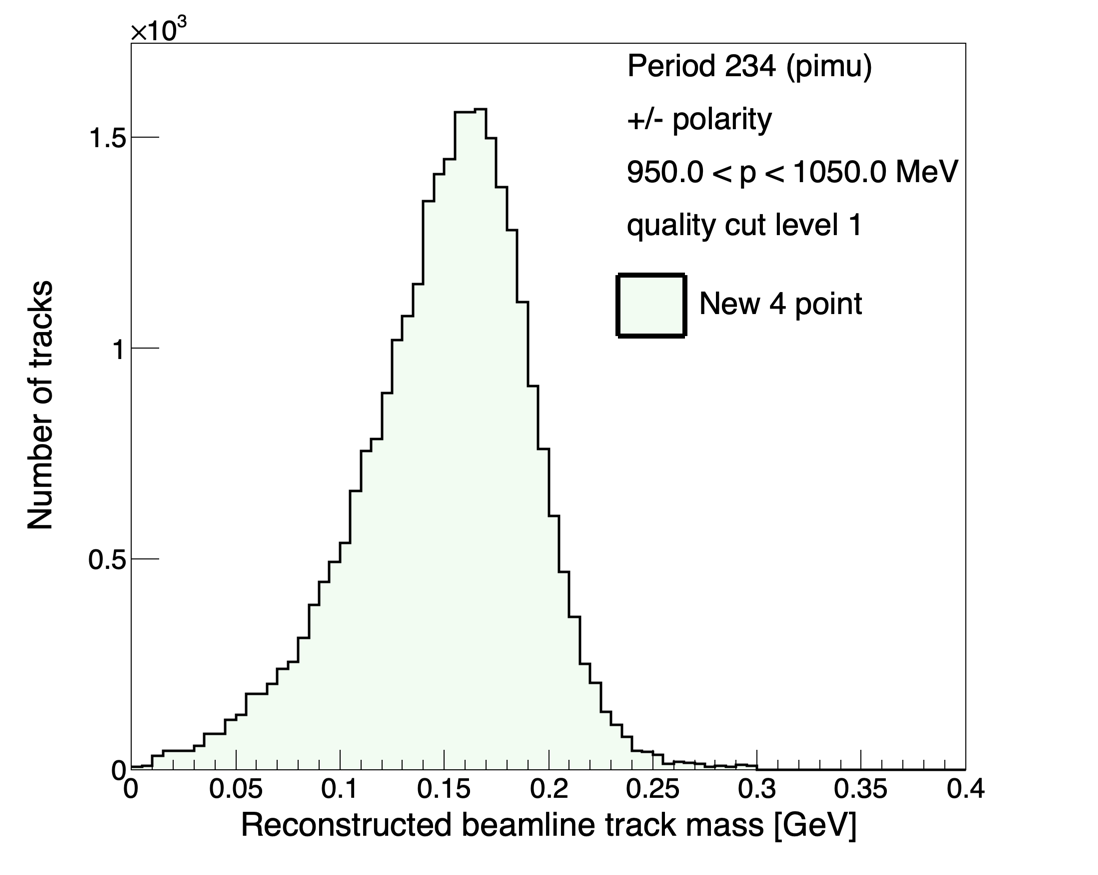
\includegraphics[width=\textwidth]{pimu_period234_mass_level0_posneg_stats_Mom1000.0_Cur1.png}
            \caption{1000 A}
            \label{fig_mpimu1000}
            \end{subfigure}
             \hfill                             
             \begin{subfigure}[b]{0.24\textwidth}
            \centering
            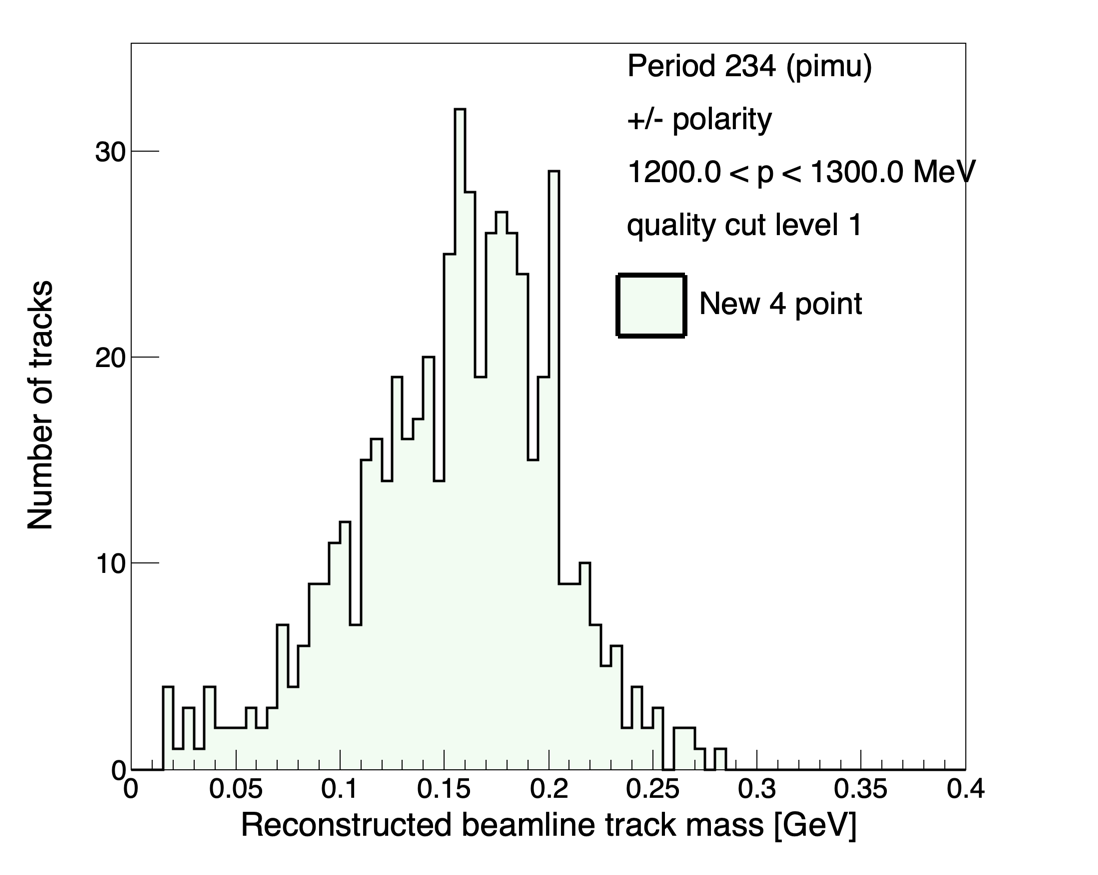
\includegraphics[width=\textwidth]{pimu_period234_mass_level0_posneg_stats_Mom1250.0_Cur1.png}
            \caption{1250 A}
            \label{fig_mpimu1250}
            \end{subfigure}
            
             \begin{subfigure}[b]{0.24\textwidth}
            \centering
            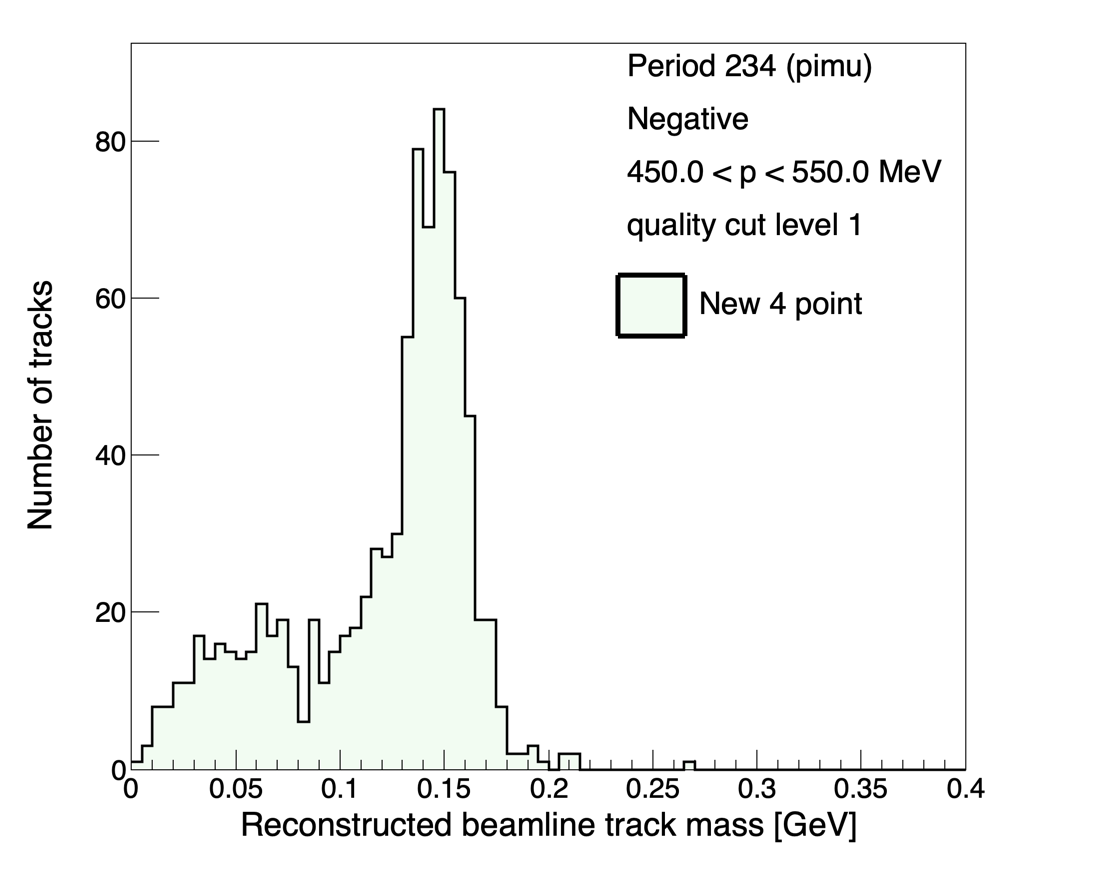
\includegraphics[width=\textwidth]{pimu_period234_mass_level0_neg_stats_Mom500.0_Cur1.png}
            \caption{-500 A}
            \label{fig_mpimu500}
            \end{subfigure}
             \hfill   
            \begin{subfigure}[b]{0.24\textwidth}
            \centering
            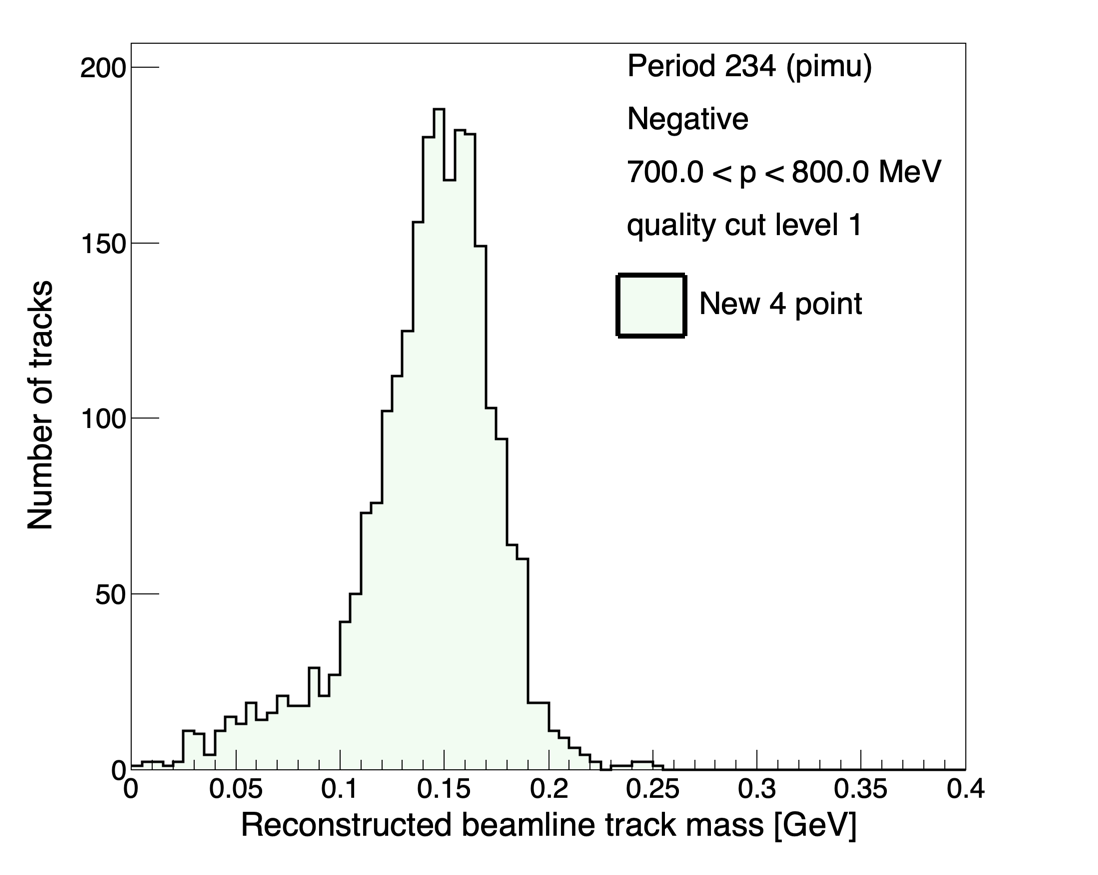
\includegraphics[width=\textwidth]{pimu_period234_mass_level0_neg_stats_Mom750.0_Cur1.png}
            \caption{-750 A}
            \label{fig_mpimu750}
            \end{subfigure}
             \hfill   
            \begin{subfigure}[b]{0.24\textwidth}
            \centering
            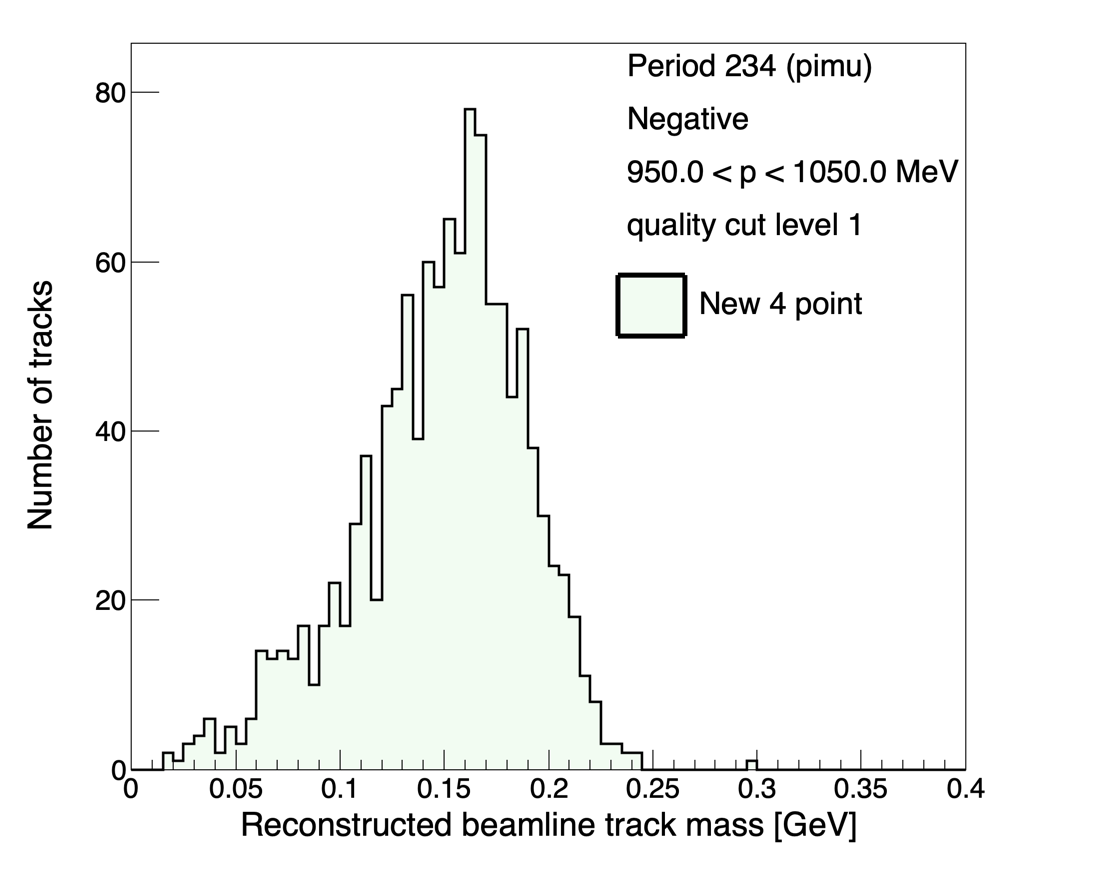
\includegraphics[width=\textwidth]{pimu_period234_mass_level0_neg_stats_Mom1000.0_Cur1.png}
            \caption{-1000 A}
            \label{fig_mpimu1000}
            \end{subfigure}
             \hfill                             
             \begin{subfigure}[b]{0.24\textwidth}
            \centering
            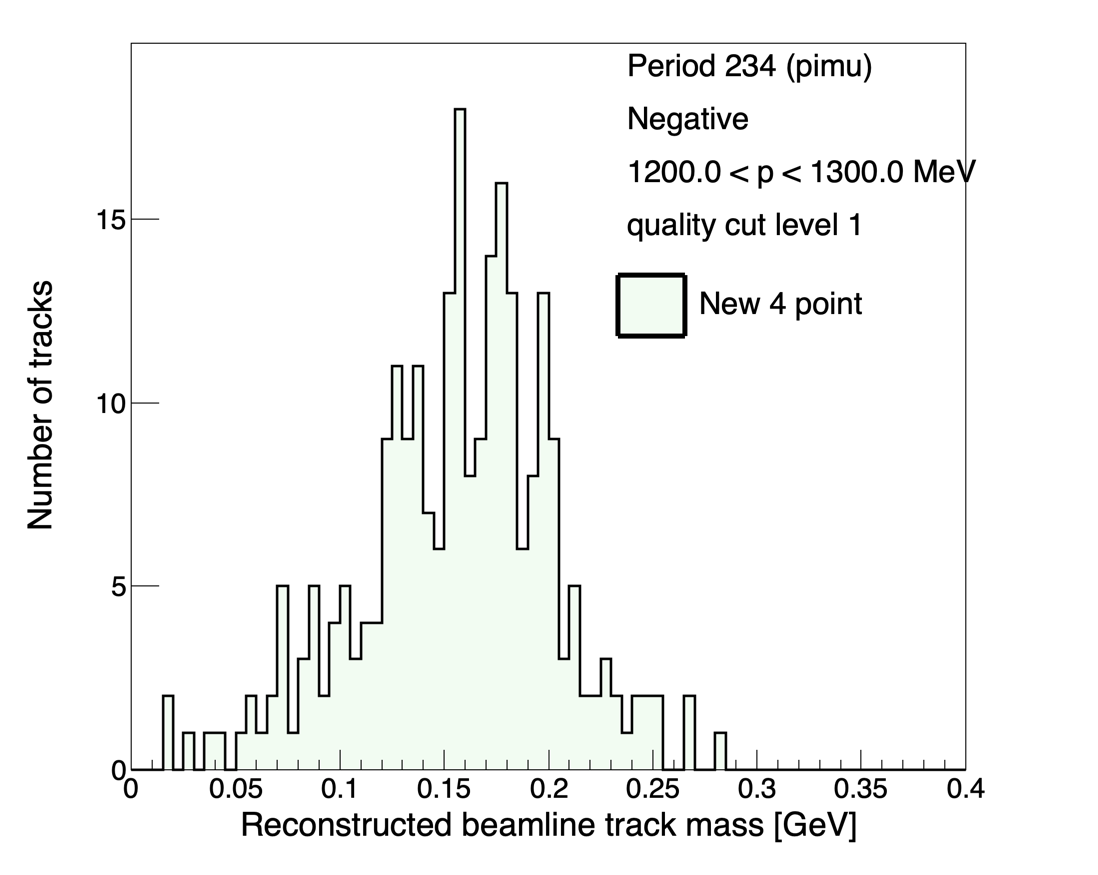
\includegraphics[width=\textwidth]{pimu_period234_mass_level0_neg_stats_Mom1250.0_Cur1.png}
            \caption{-1250 A}
            \label{fig_mpimu-1250}
            \end{subfigure}
            
            \begin{subfigure}[b]{0.24\textwidth}
            \centering
            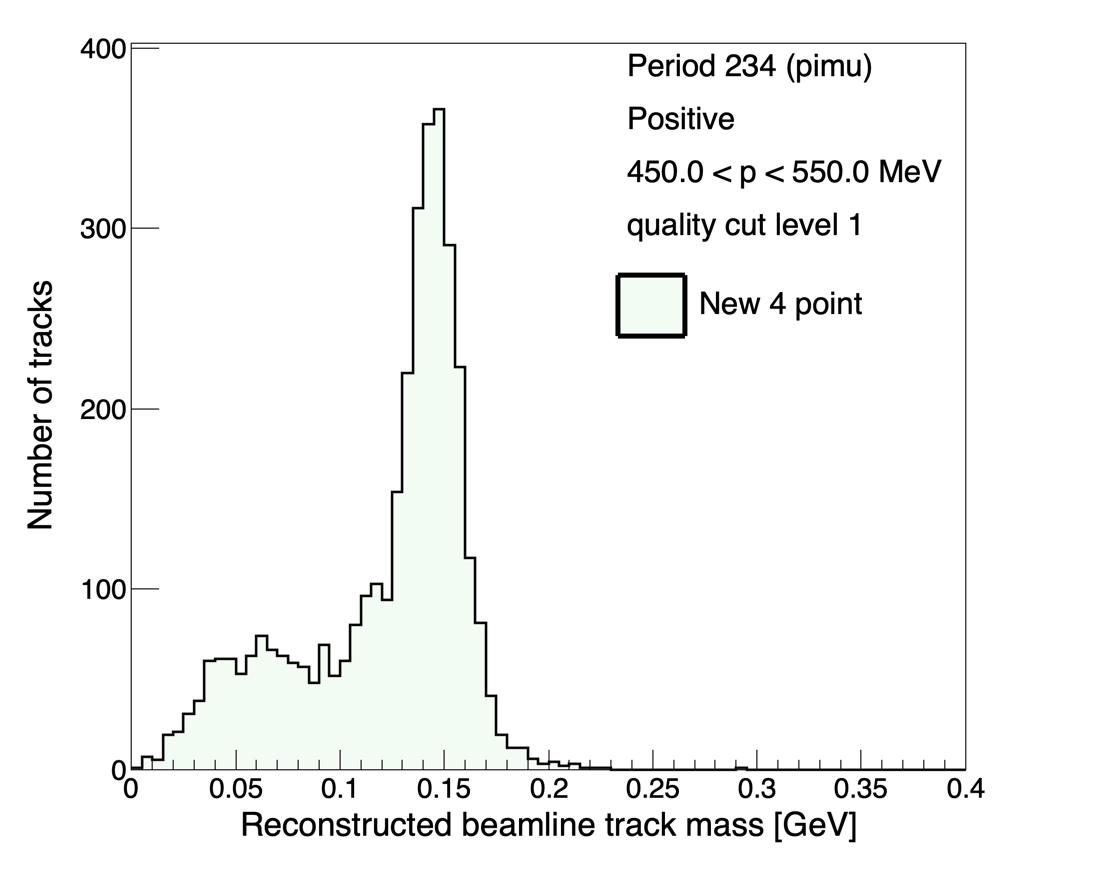
\includegraphics[width=\textwidth]{pimu_period234_mass_level0_pos_stats_Mom500.0_Cur1.png}
            \caption{+500 A}
            \label{fig_mpimu+500}
            \end{subfigure}
             \hfill   
            \begin{subfigure}[b]{0.24\textwidth}
            \centering
            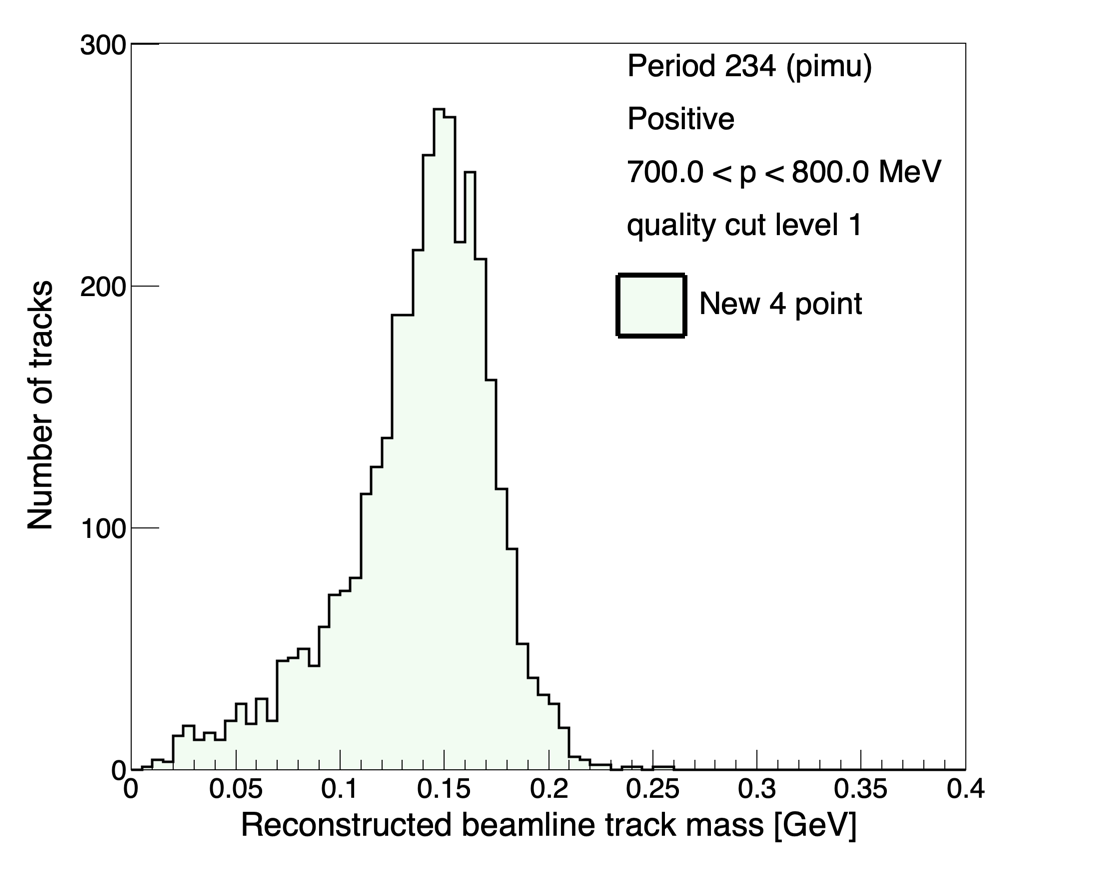
\includegraphics[width=\textwidth]{pimu_period234_mass_level0_pos_stats_Mom750.0_Cur1.png}
            \caption{+750 A}
            \label{fig_mpimu+750}
            \end{subfigure}
             \hfill   
            \begin{subfigure}[b]{0.24\textwidth}
            \centering
            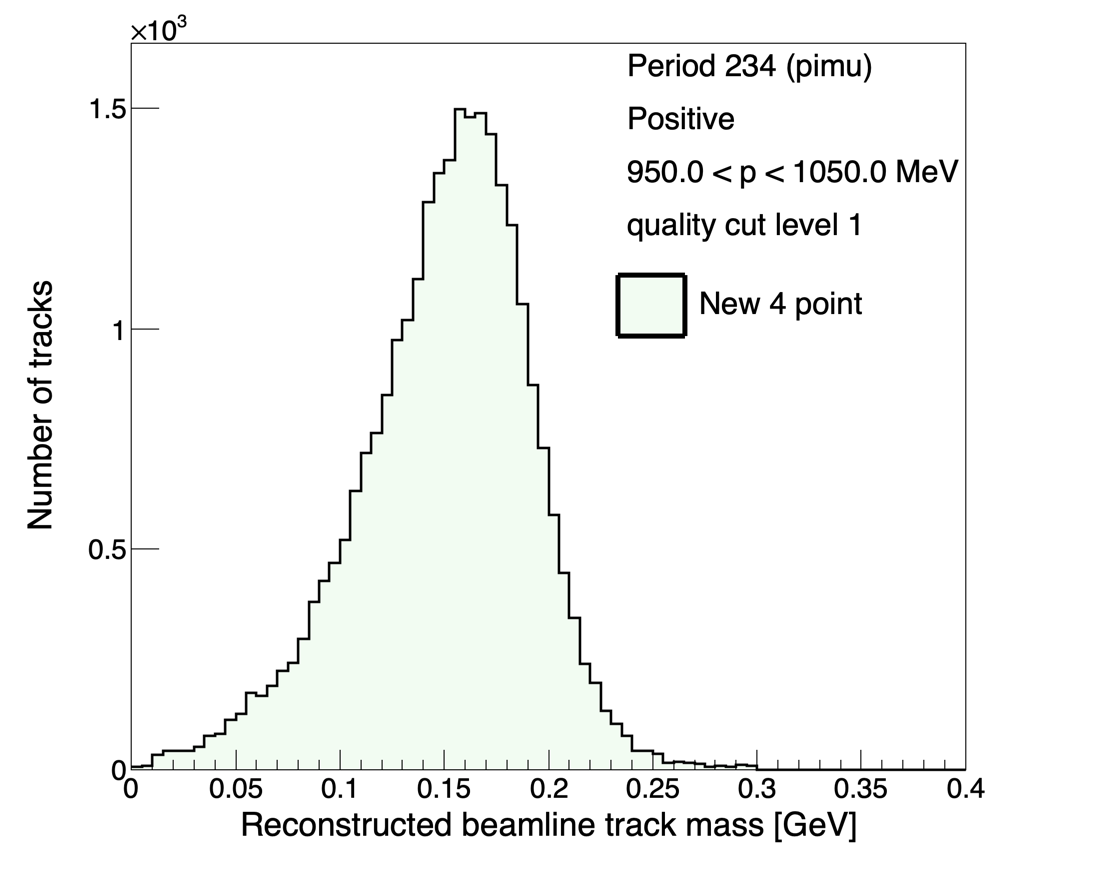
\includegraphics[width=\textwidth]{pimu_period234_mass_level0_pos_stats_Mom1000.0_Cur1.png}
            \caption{+1000 A}
            \label{fig_mpimu+1000}
            \end{subfigure}
             \hfill                             
             \begin{subfigure}[b]{0.24\textwidth}
            \centering
            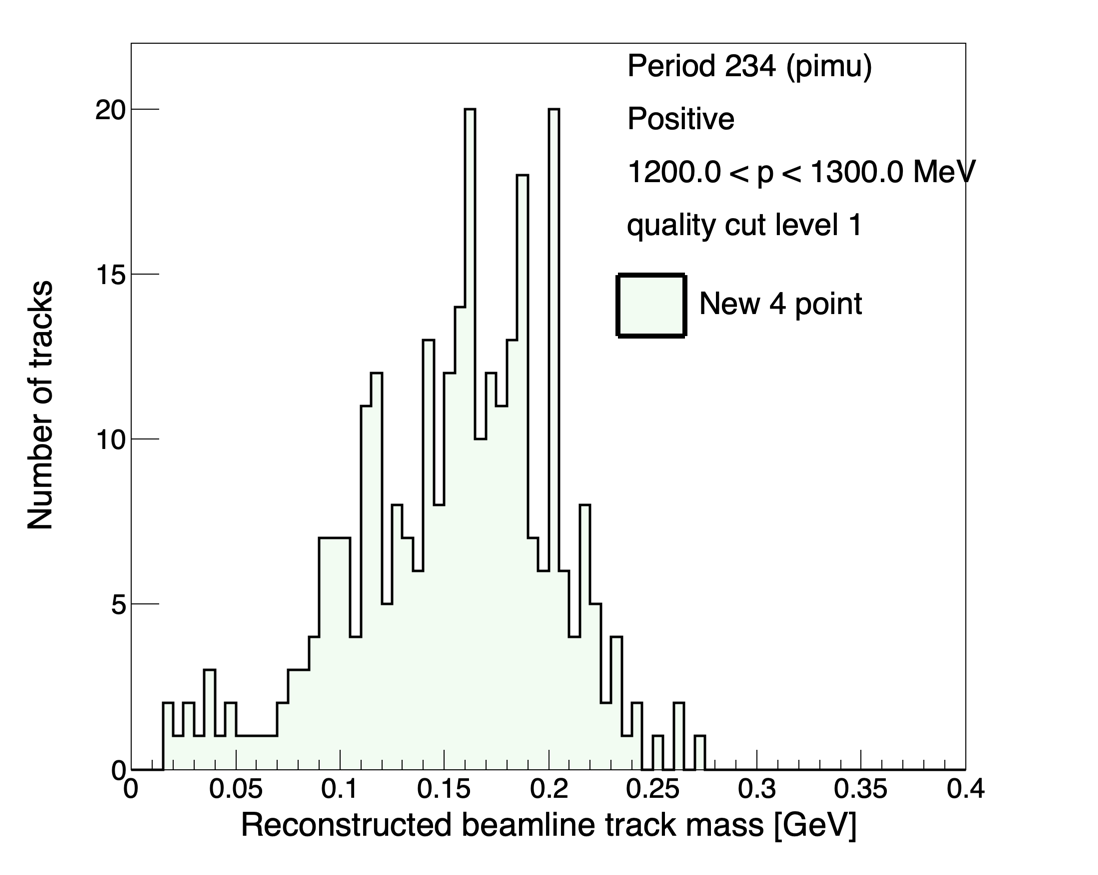
\includegraphics[width=\textwidth]{pimu_period234_mass_level0_pos_stats_Mom1250.0_Cur1.png}
            \caption{+1250 A}
            \label{fig_mpimu+1250}
            \end{subfigure}
                        
\caption{The mass distribution in the region of the pion mass for different magnet current settings shows the distribution widening significantly as the momentum increases. The bottom row shows the distributions with negative polarity. Level 1 means that there are no cuts applied other than the requirement that the momentum is consistent with the magnet current.} 
\label{fig_pimumass}
  \end{figure}
 

 \begin{figure}[h]	
 \centering   
            \begin{subfigure}[b]{0.24\textwidth}
            \centering
            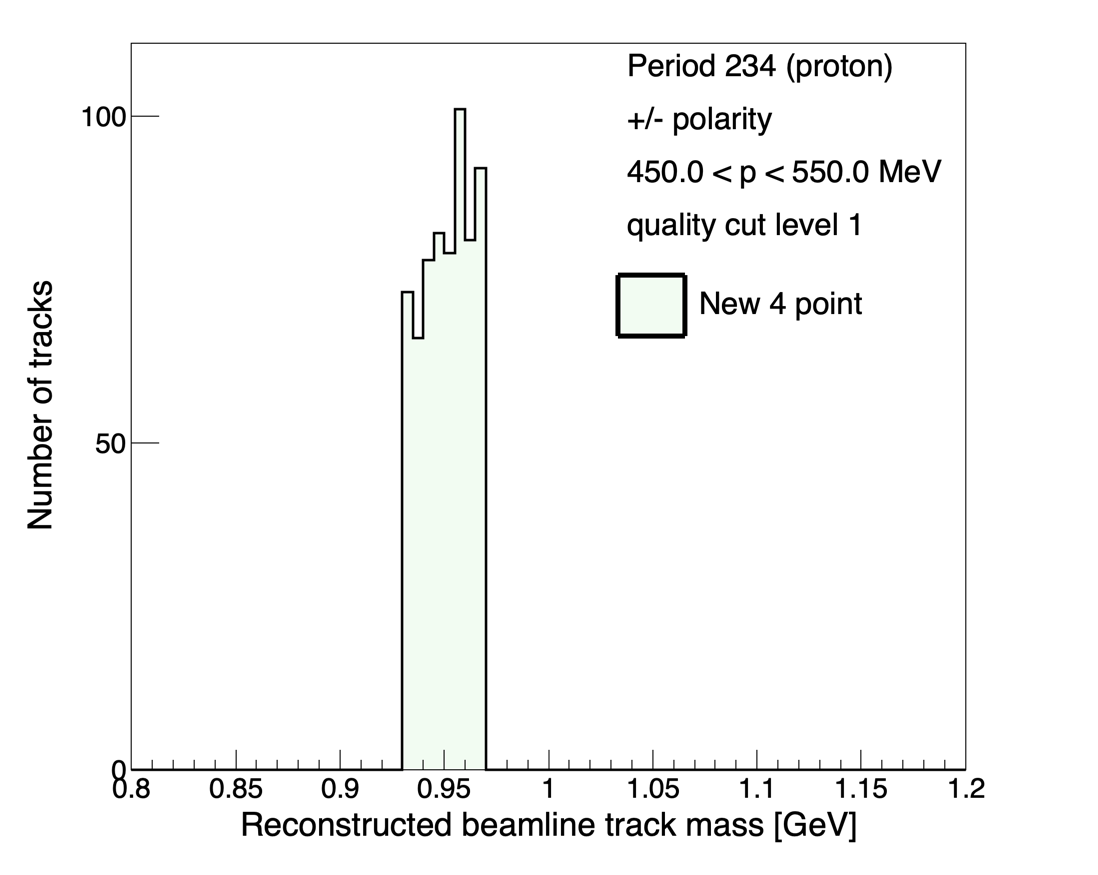
\includegraphics[width=\textwidth]{proton_period234_mass_level0_posneg_stats_Mom500.0_Cur1.png}
            \caption{500 A}
            \label{fig_mproton500}
            \end{subfigure}
             \hfill   
            \begin{subfigure}[b]{0.24\textwidth}
            \centering
            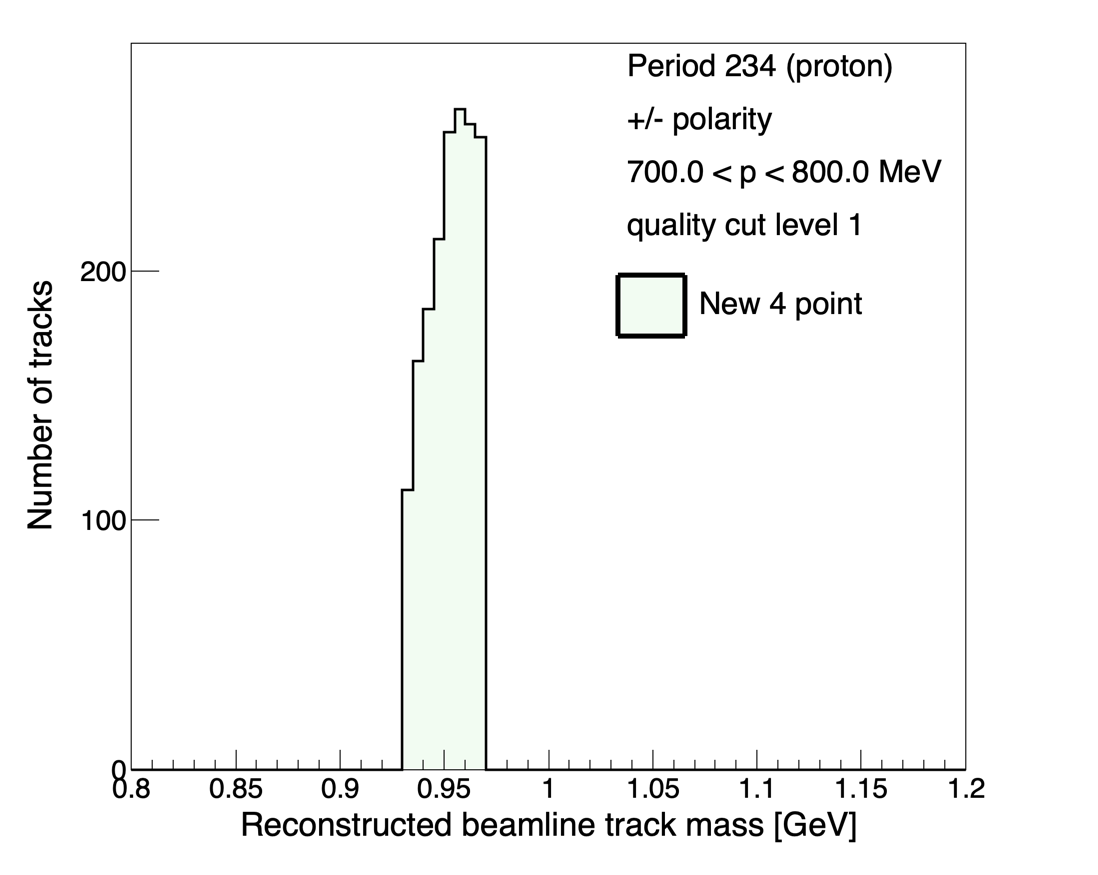
\includegraphics[width=\textwidth]{proton_period234_mass_level0_posneg_stats_Mom750.0_Cur1.png}
            \caption{750 A}
            \label{fig_mproton750}
            \end{subfigure}
             \hfill   
            \begin{subfigure}[b]{0.24\textwidth}
            \centering
            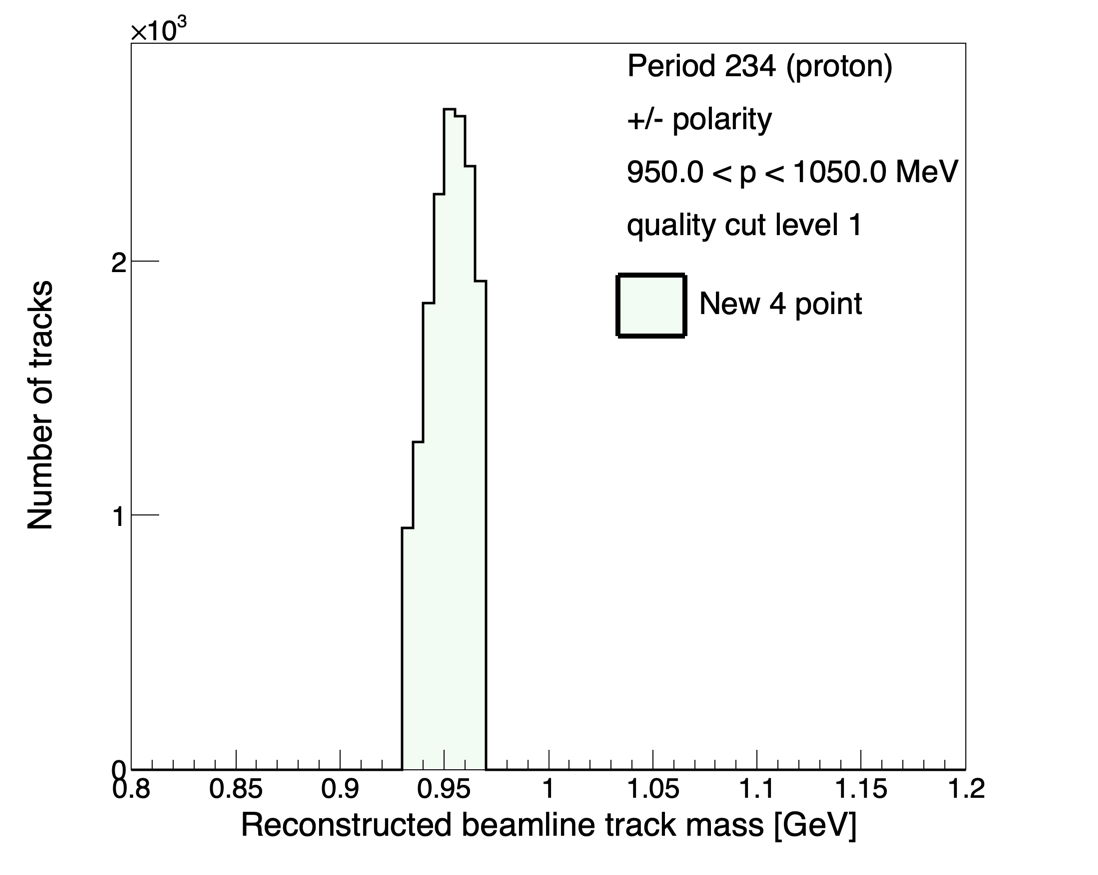
\includegraphics[width=\textwidth]{proton_period234_mass_level0_posneg_stats_Mom1000.0_Cur1.png}
            \caption{1000 A}
            \label{fig_mproton1000}
            \end{subfigure}
             \hfill                             
             \begin{subfigure}[b]{0.24\textwidth}
            \centering
            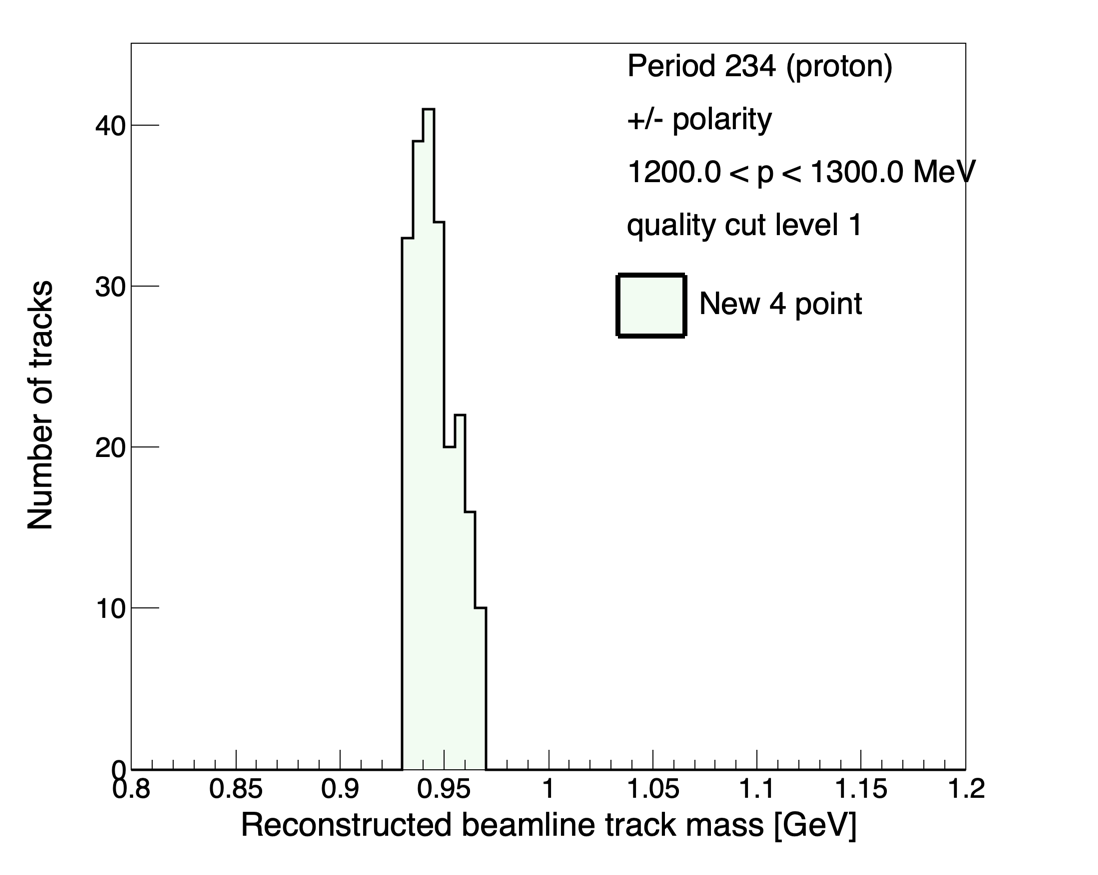
\includegraphics[width=\textwidth]{proton_period234_mass_level0_posneg_stats_Mom1250.0_Cur1.png}
            \caption{1250 A}
            \label{fig_mproton1250}
            \end{subfigure}
            
                        \begin{subfigure}[b]{0.24\textwidth}
            \centering
            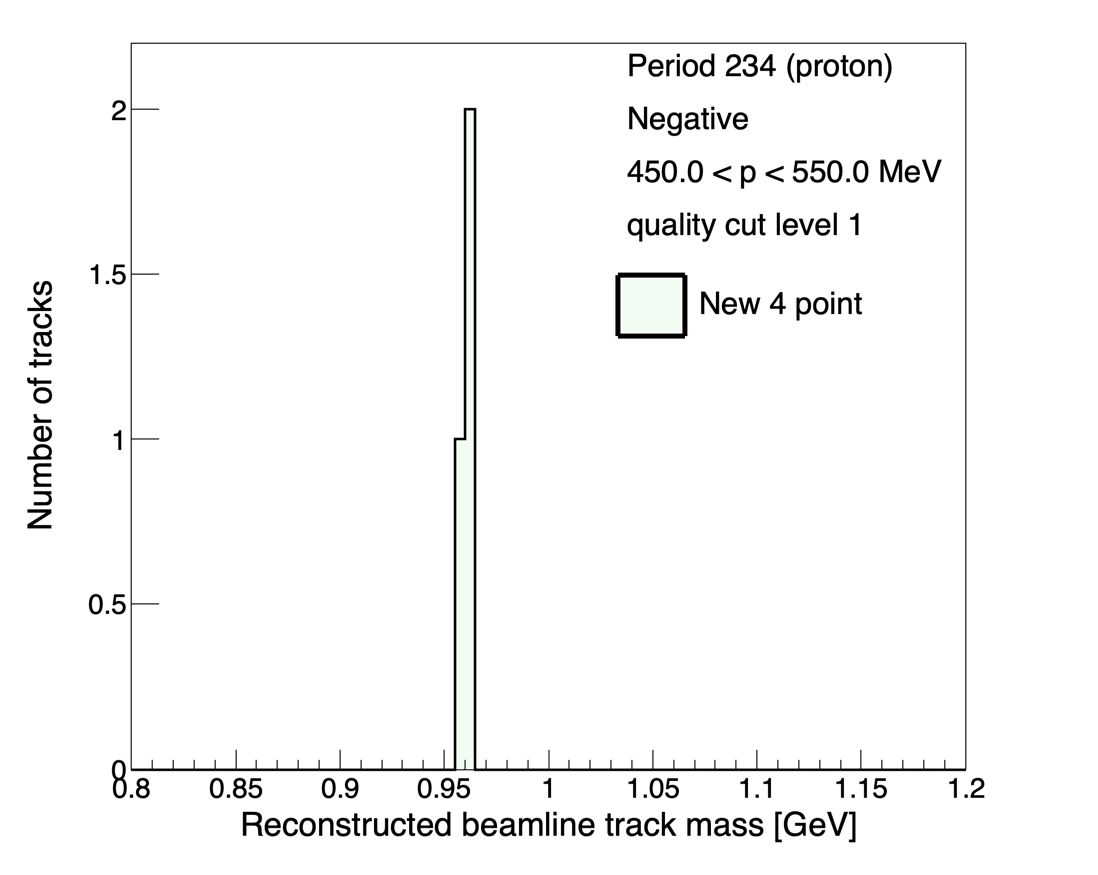
\includegraphics[width=\textwidth]{proton_period234_mass_level0_neg_stats_Mom500.0_Cur1.png}
            \caption{-500 A}
            \label{fig_mproton-500}
            \end{subfigure}
             \hfill   
            \begin{subfigure}[b]{0.24\textwidth}
            \centering
            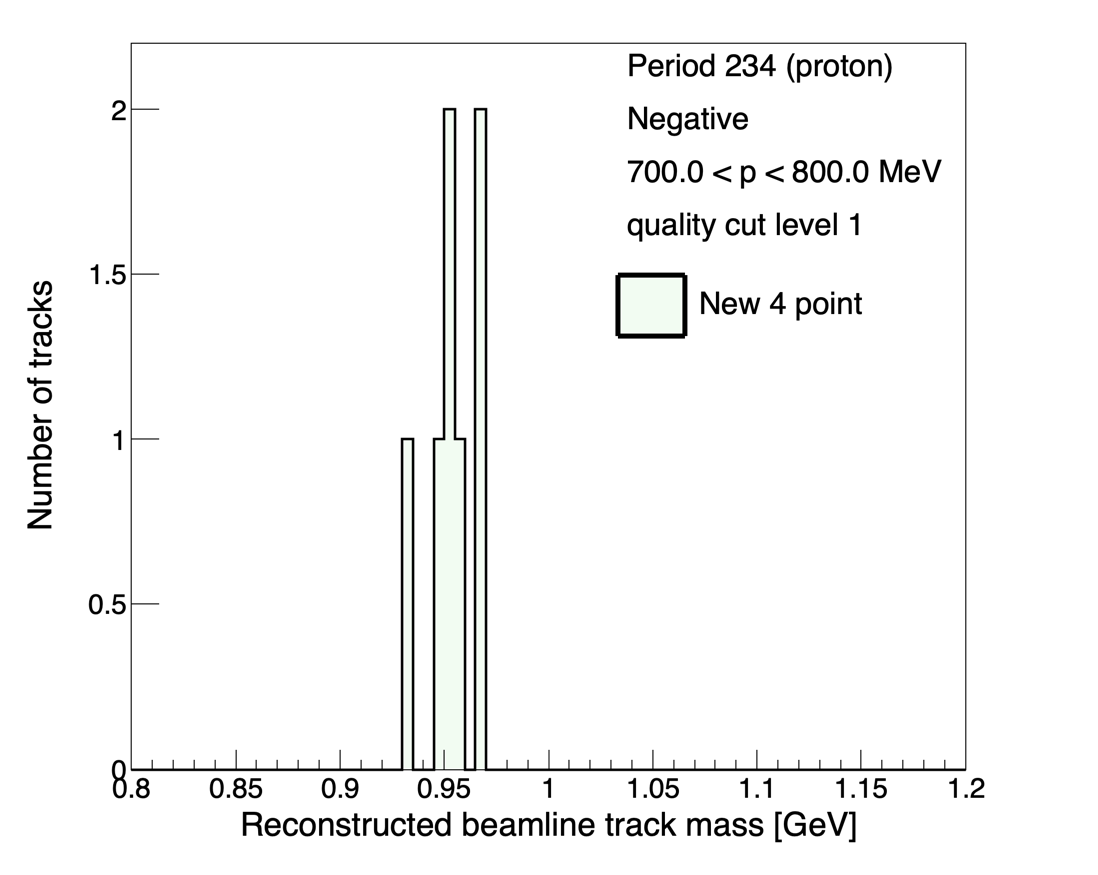
\includegraphics[width=\textwidth]{proton_period234_mass_level0_neg_stats_Mom750.0_Cur1.png}
            \caption{-750 A}
            \label{fig_mproton-750}
            \end{subfigure}
             \hfill   
            \begin{subfigure}[b]{0.24\textwidth}
            \centering
            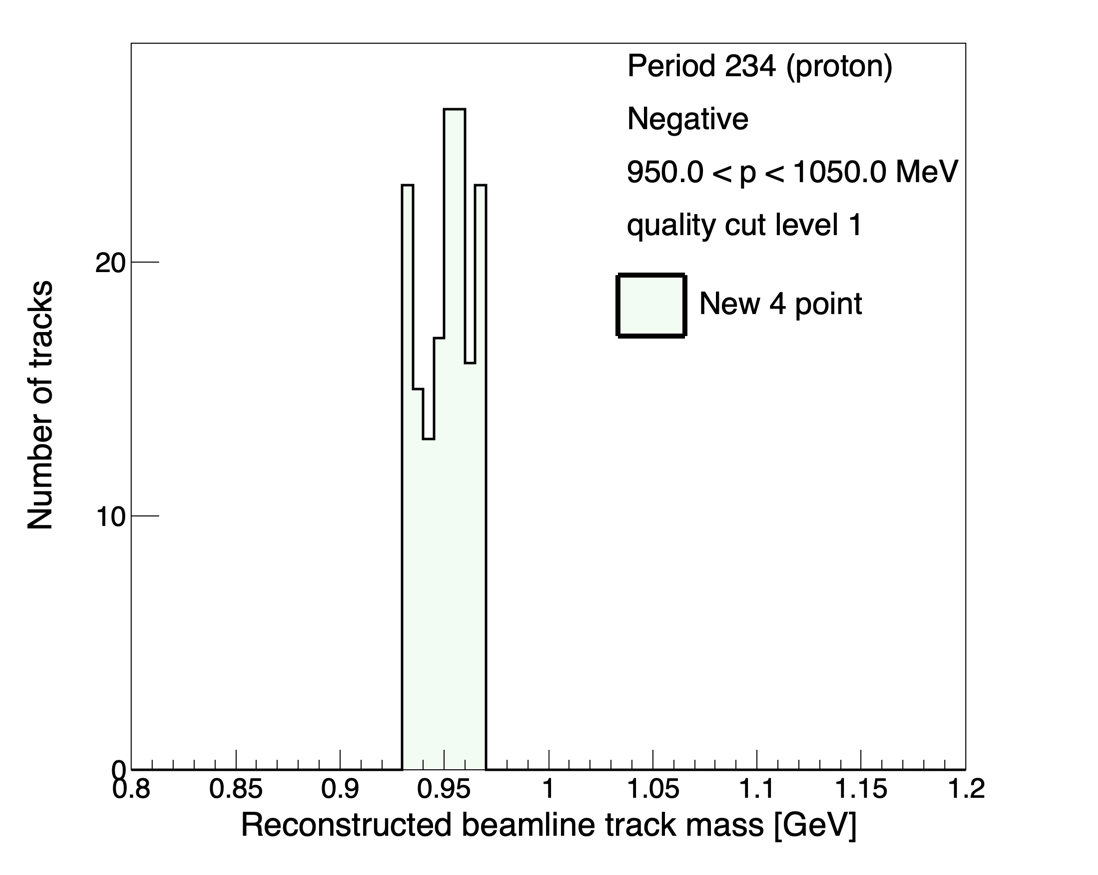
\includegraphics[width=\textwidth]{proton_period234_mass_level0_neg_stats_Mom1000.0_Cur1.png}
            \caption{-1000 A}
            \label{fig_mproton-1000}
            \end{subfigure}
             \hfill                             
             \begin{subfigure}[b]{0.24\textwidth}
            \centering
            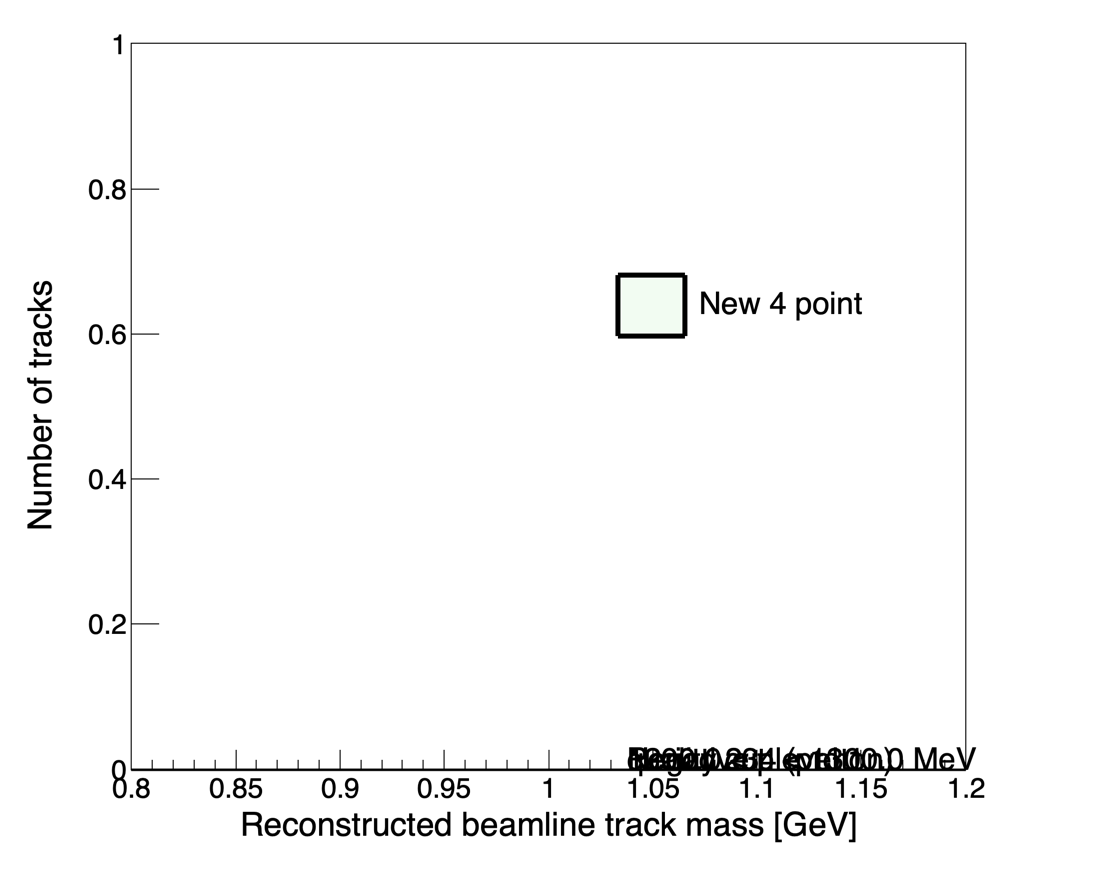
\includegraphics[width=\textwidth]{proton_period234_mass_level0_neg_stats_Mom1250.0_Cur1.png}
            \caption{-1250 A}
            \label{fig_mproton-1250}
            \end{subfigure}
            
             \begin{subfigure}[b]{0.24\textwidth}
            \centering
            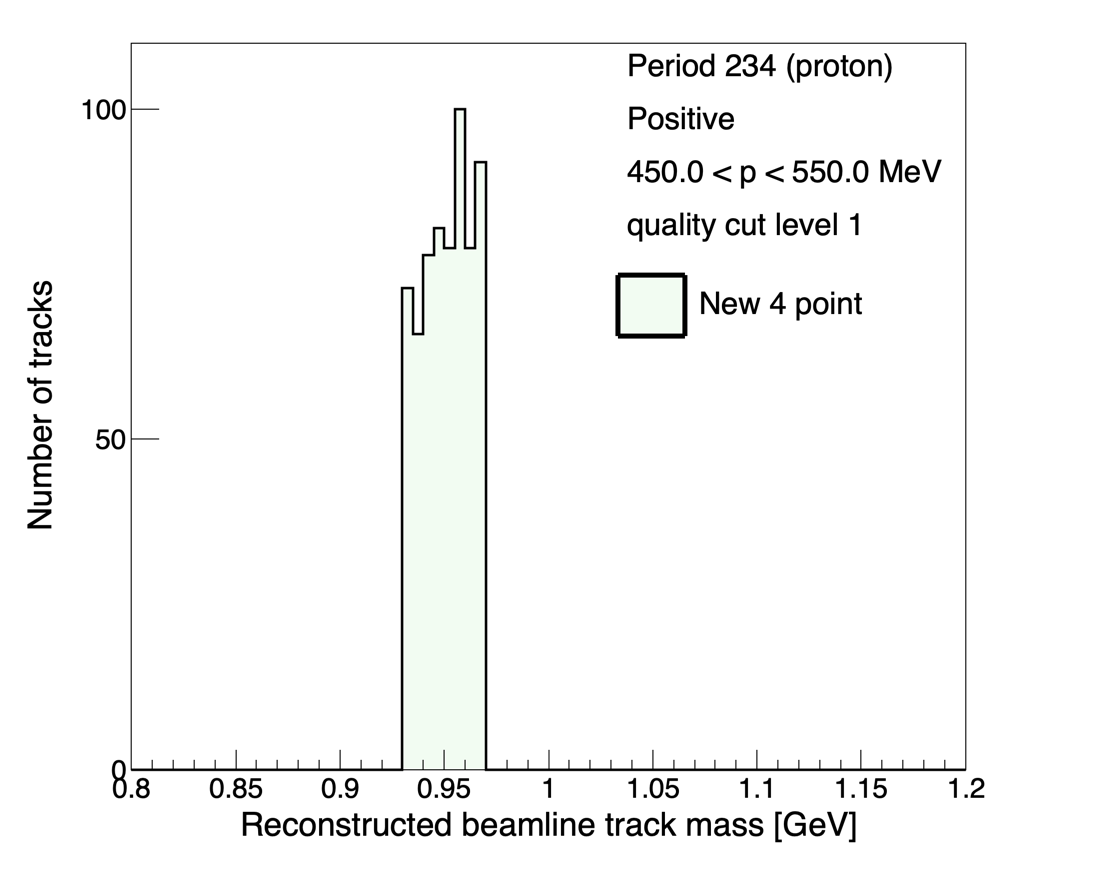
\includegraphics[width=\textwidth]{proton_period234_mass_level0_pos_stats_Mom500.0_Cur1.png}
            \caption{+500 A}
            \label{fig_mproton500}
            \end{subfigure}
             \hfill   
            \begin{subfigure}[b]{0.24\textwidth}
            \centering
            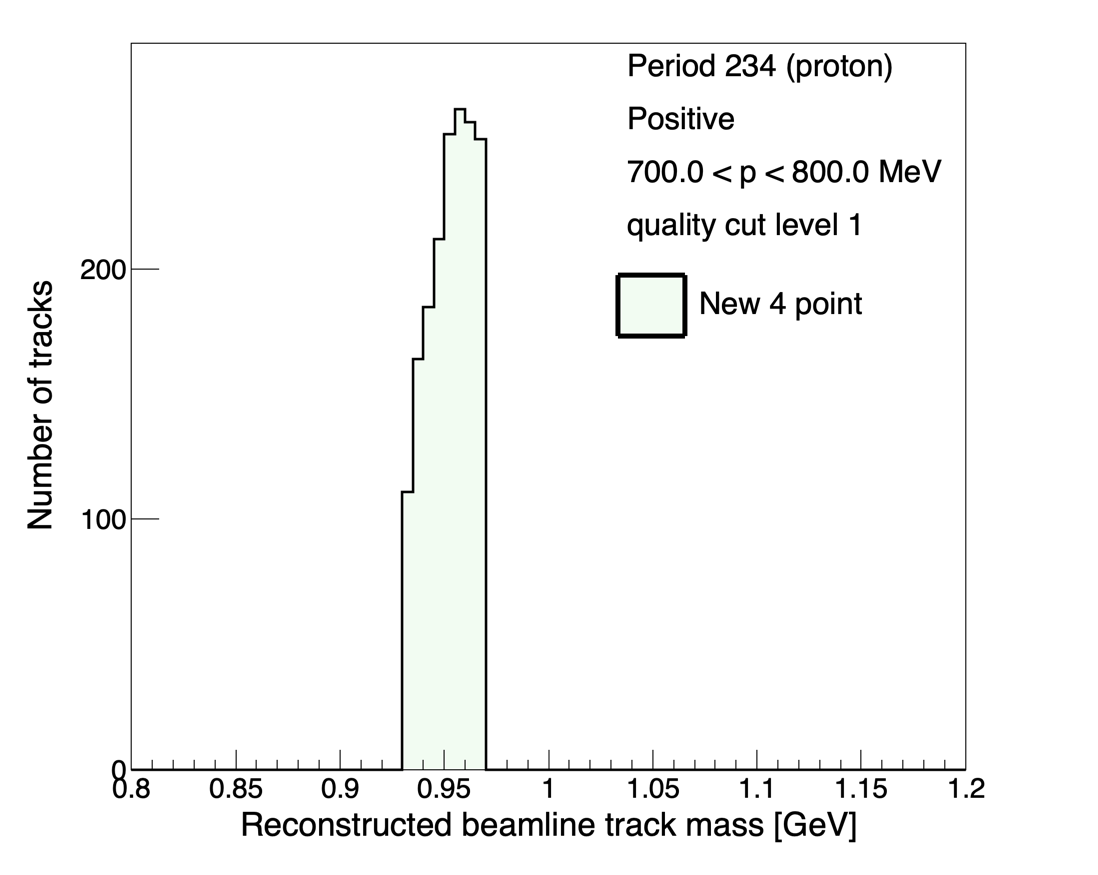
\includegraphics[width=\textwidth]{proton_period234_mass_level0_pos_stats_Mom750.0_Cur1.png}
            \caption{+750 A}
            \label{fig_mproton750}
            \end{subfigure}
             \hfill   
            \begin{subfigure}[b]{0.24\textwidth}
            \centering
            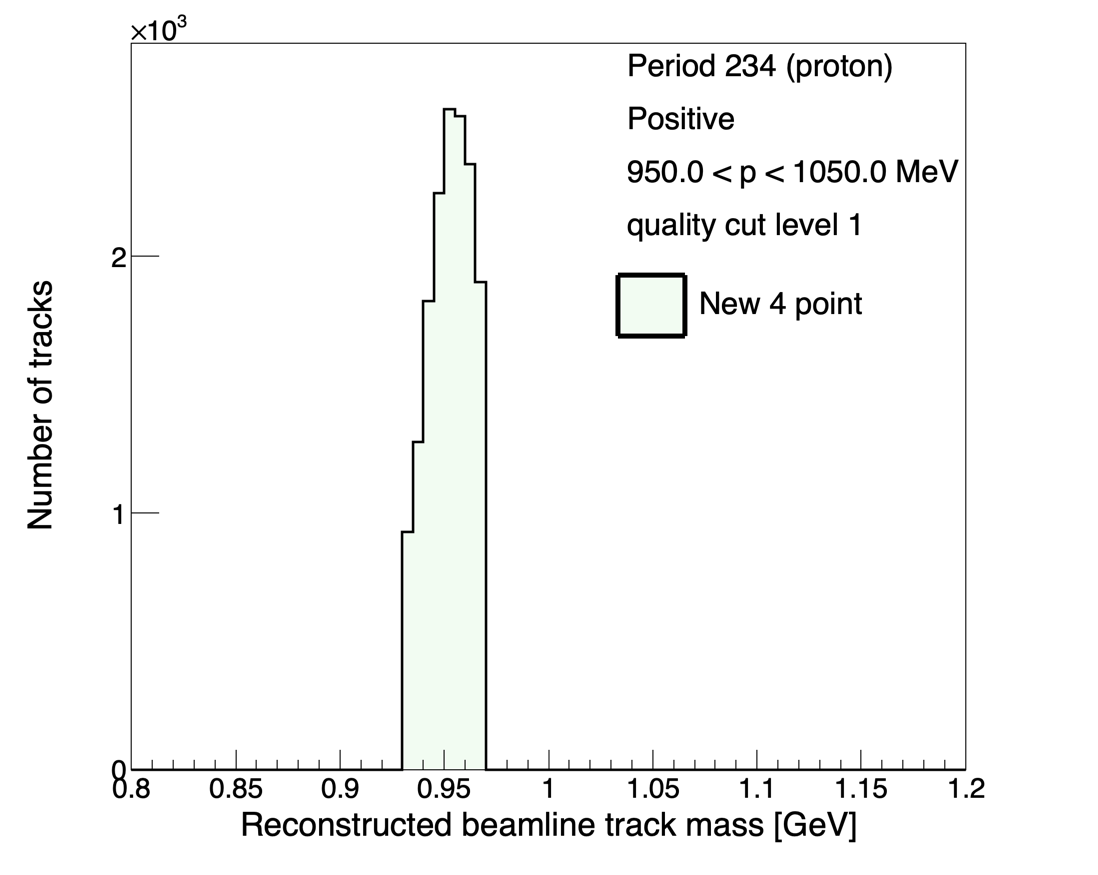
\includegraphics[width=\textwidth]{proton_period234_mass_level0_pos_stats_Mom1000.0_Cur1.png}
            \caption{+1000 A}
            \label{fig_mproton1000}
            \end{subfigure}
             \hfill                             
             \begin{subfigure}[b]{0.24\textwidth}
            \centering
            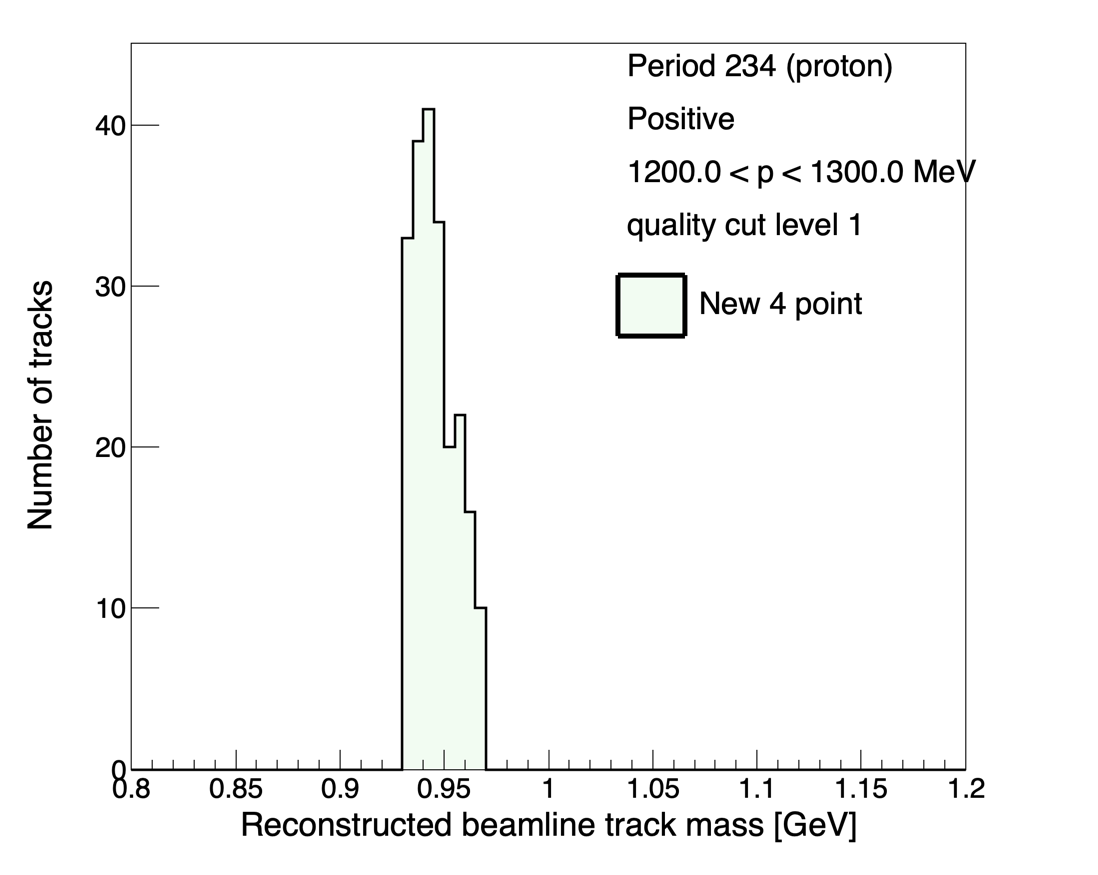
\includegraphics[width=\textwidth]{proton_period234_mass_level0_pos_stats_Mom1250.0_Cur1.png}
            \caption{+1250 A}
            \label{fig_mproton+1250}
            \end{subfigure}

            
\caption{The mass distribution in the region of the proton mass for different magnet current settings. Level 1 means that there are no cuts applied other than the requirement that the momentum is consistent with the magnet current.} 
\label{fig_protonmass}
  \end{figure}
  
  \newpage
  
  \subsection{Particle speeds}
  
  Looking at the particle speeds for different particles can help us to figure out how much we trust the time of flight measurements and is just interesting in its own right.
  
   \begin{figure}[h]	
 \centering   
               \begin{subfigure}[b]{0.3\textwidth}
            \centering
            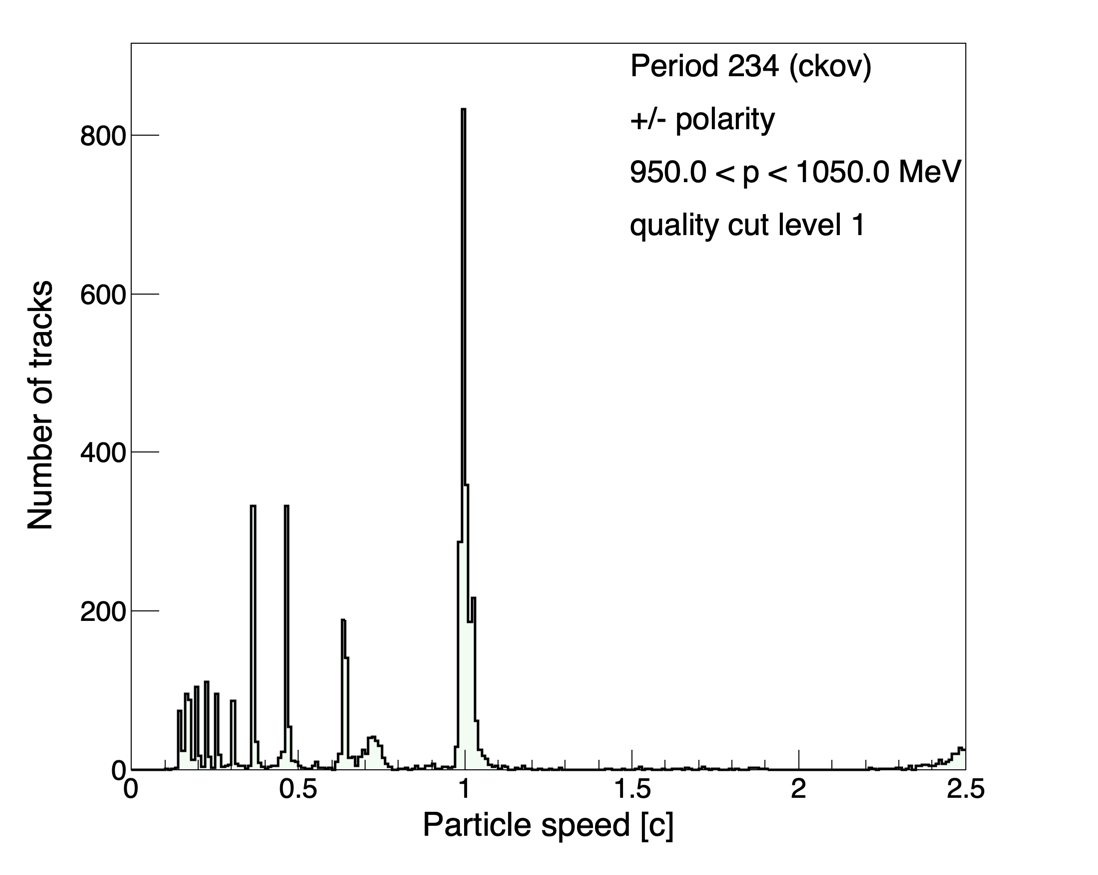
\includegraphics[width=\textwidth]{ckov_period234_beta_level0_posneg_stats_Mom1000.0_Cur1.png}
            \caption{1000 A}
           % \label{fig_mproton500}
            \end{subfigure}
             \hfill   
            \begin{subfigure}[b]{0.3\textwidth}
            \centering
            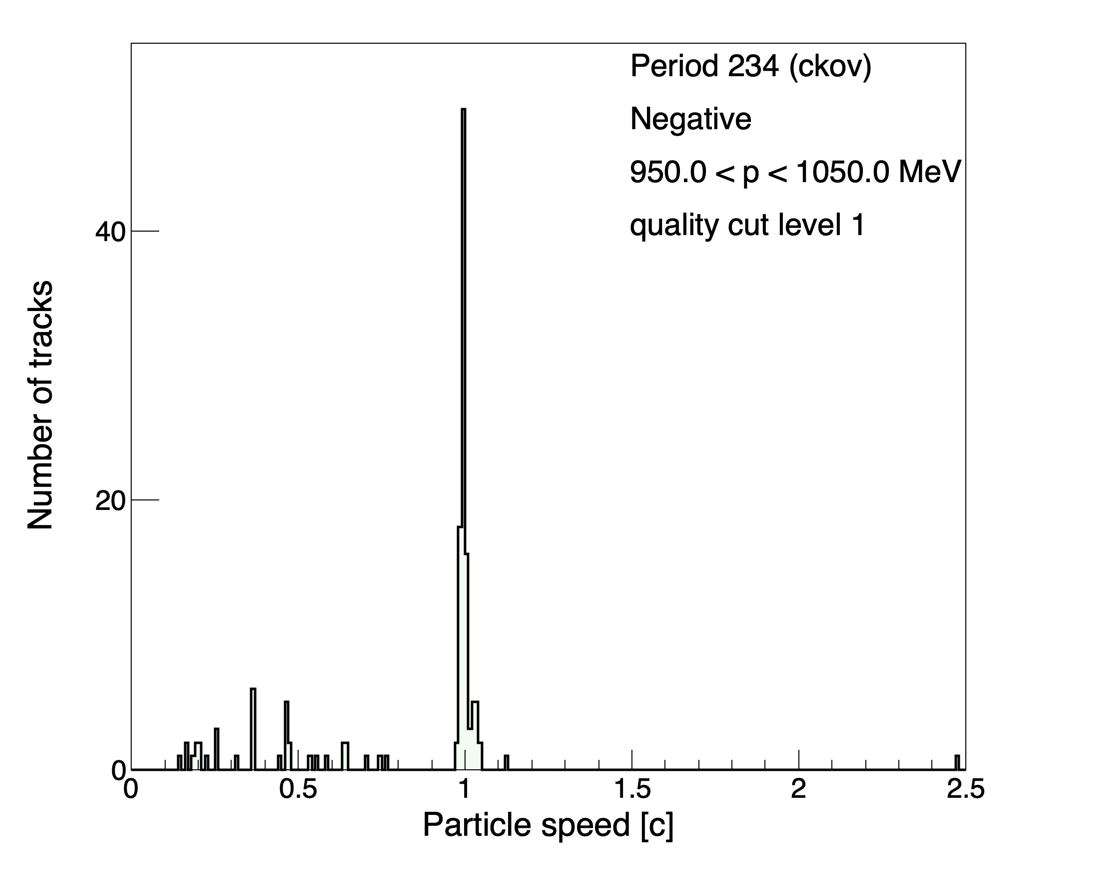
\includegraphics[width=\textwidth]{ckov_period234_beta_level0_neg_stats_Mom1000.0_Cur1.png}
            \caption{+1000 A}
            %\label{fig_mproton750}
            \end{subfigure}
             \hfill   
            \begin{subfigure}[b]{0.3\textwidth}
            \centering
            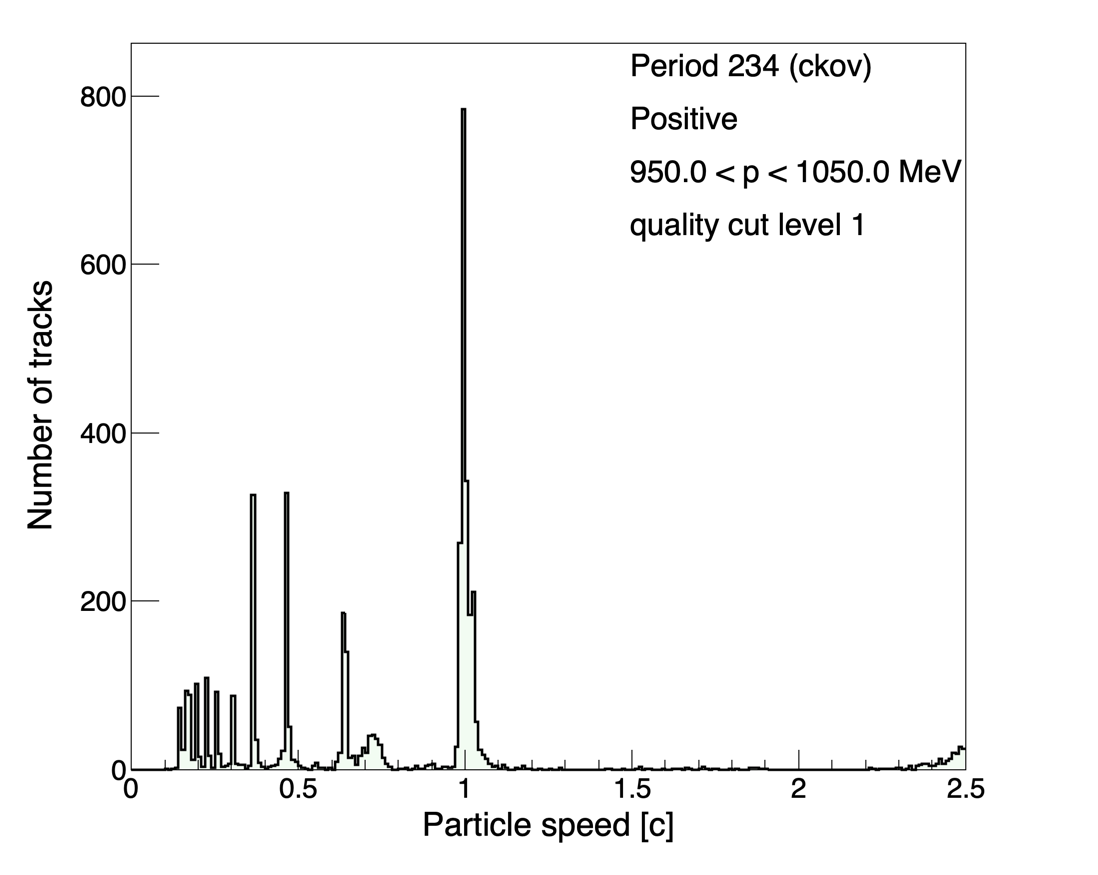
\includegraphics[width=\textwidth]{ckov_period234_beta_level0_pos_stats_Mom1000.0_Cur1.png}
            \caption{-1000 A}
           % \label{fig_mproton1000}
            \end{subfigure}
  

            
\caption{The speed of candidate particles that leave a signal in the threshold cherenkov detector. Everything in the big peak near the speed of light has a negligible wirechamber mass making it likely that these are indeed electrons. The hillock next on the left is consistent with the proton mass, something is happening between the proton leaving the wirechambers and entering the ckov  to get a ckov signal? I think that the beats at lower speeds are instrumental features.  }
\label{fig_beta-ckov}
  \end{figure}
  

   \begin{figure}[h]	
 \centering   
               \begin{subfigure}[b]{0.3\textwidth}
            \centering
            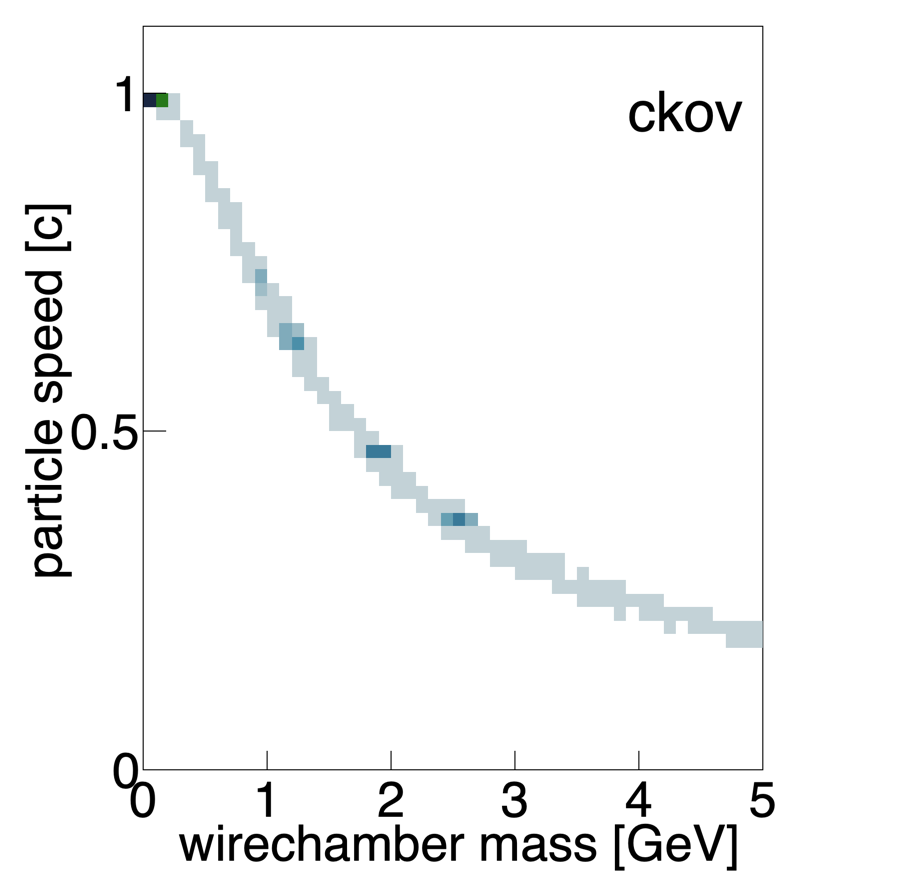
\includegraphics[width=\textwidth]{ckov_mass-v-beta_pol-1_period234cur1000.png}
            \caption{Full range}
           % \label{fig_mproton500}
            \end{subfigure}
             \hfill   
            \begin{subfigure}[b]{0.3\textwidth}
            \centering
            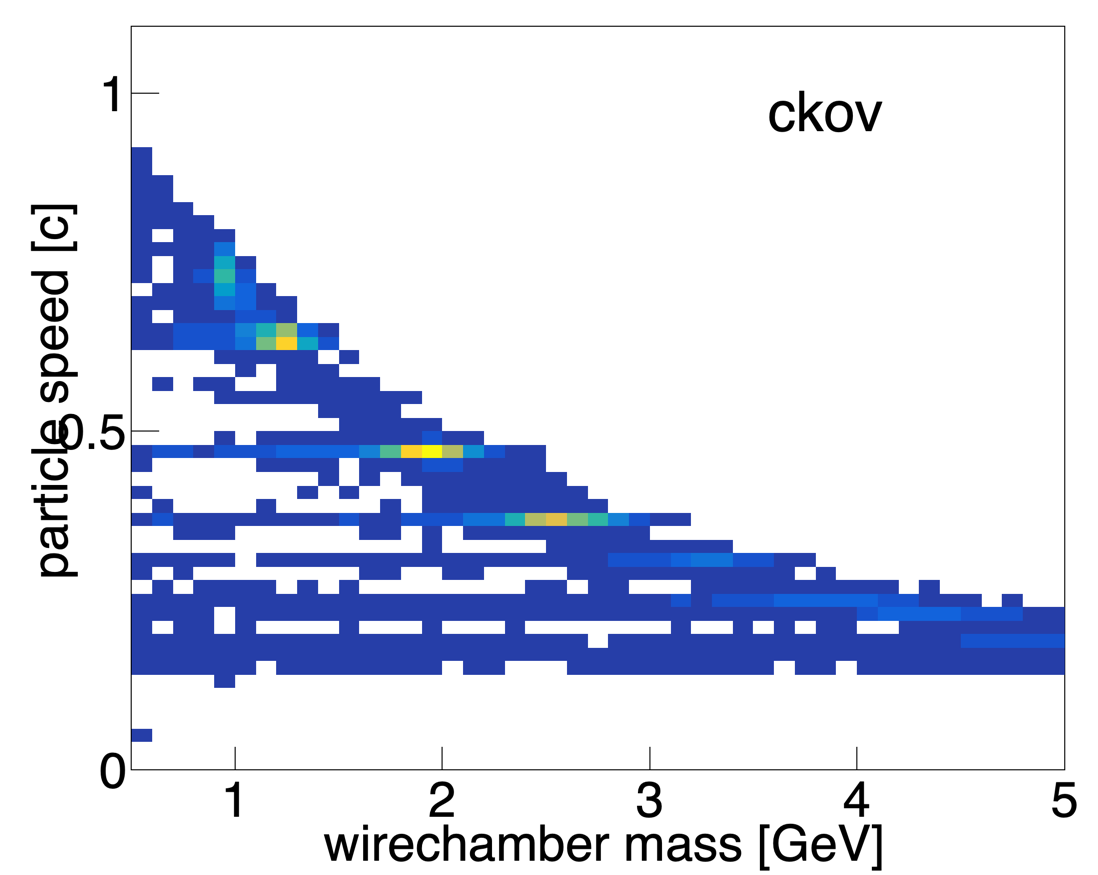
\includegraphics[width=\textwidth]{ckov_mass-v-beta_pol-1_period234cur1000-nop.png}
            \caption{Mass $>$ 0.5}
            %\label{fig_mproton750}
            \end{subfigure}
             \hfill   
            \begin{subfigure}[b]{0.3\textwidth}
            \centering
            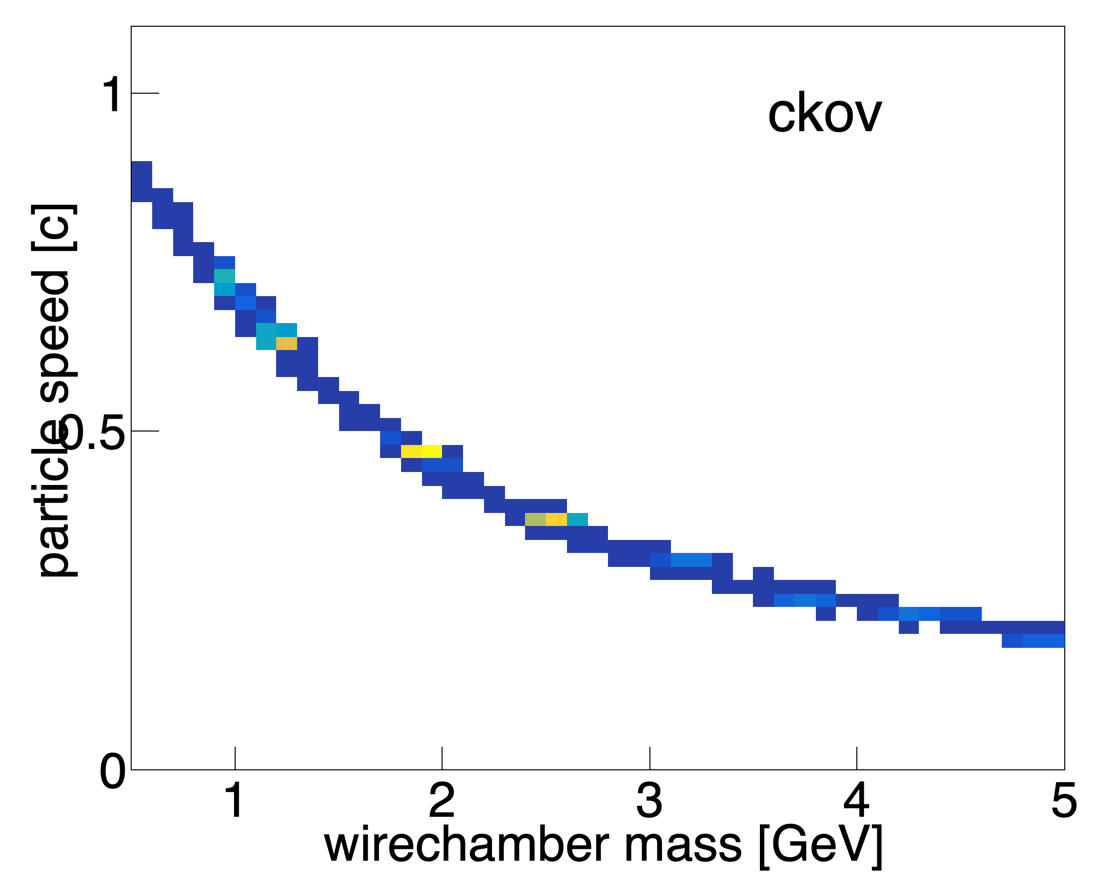
\includegraphics[width=\textwidth]{ckov_mass-v-beta_pol-1_period234cur1000-tightp.png}
            \caption{Momentum 950-1050 MeV}
           % \label{fig_mproton1000}
            \end{subfigure}
            
\caption{Speed against wirechamber mass. The left shows the full range, and is completely dominated by signals with $\beta\sim 1$ and very low wirechamber mass. Center: Removing signals with wirechamber mass less than 0.5 GeV reveals peaks at higher masses, lower speeds. These peaks look suspiciously periodic. Right: Cutting tight on momentum to remove some of the noise, the peaks are clearly visible. \textcolor{red}{Look into this suspiscion about instrumentation a bit more} }
\label{fig_beta-mass-ckov}
  \end{figure}
  
  
     \begin{figure}[h]	
 \centering   
               \begin{subfigure}[b]{0.3\textwidth}
            \centering
            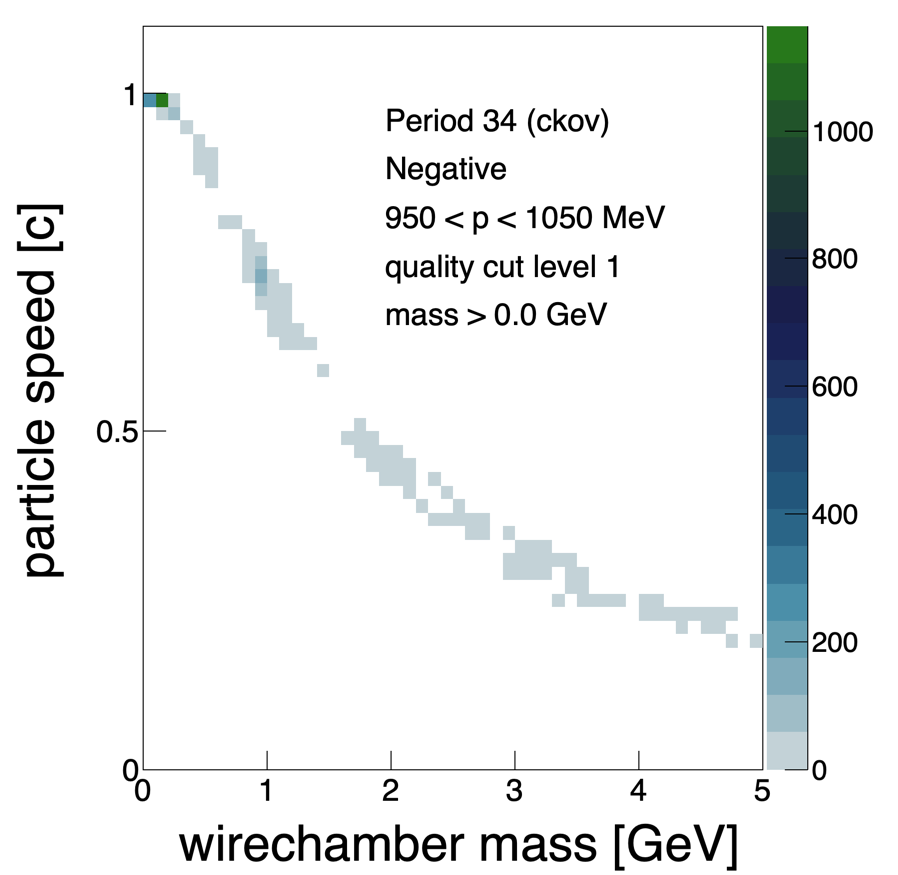
\includegraphics[width=\textwidth]{ckov_period34_mexy_level0_neg_Mom1000_Cur1_allmass.png}
            \caption{Full range}
           % \label{fig_mproton500}
            \end{subfigure}
             \hfill   
            \begin{subfigure}[b]{0.3\textwidth}
            \centering
            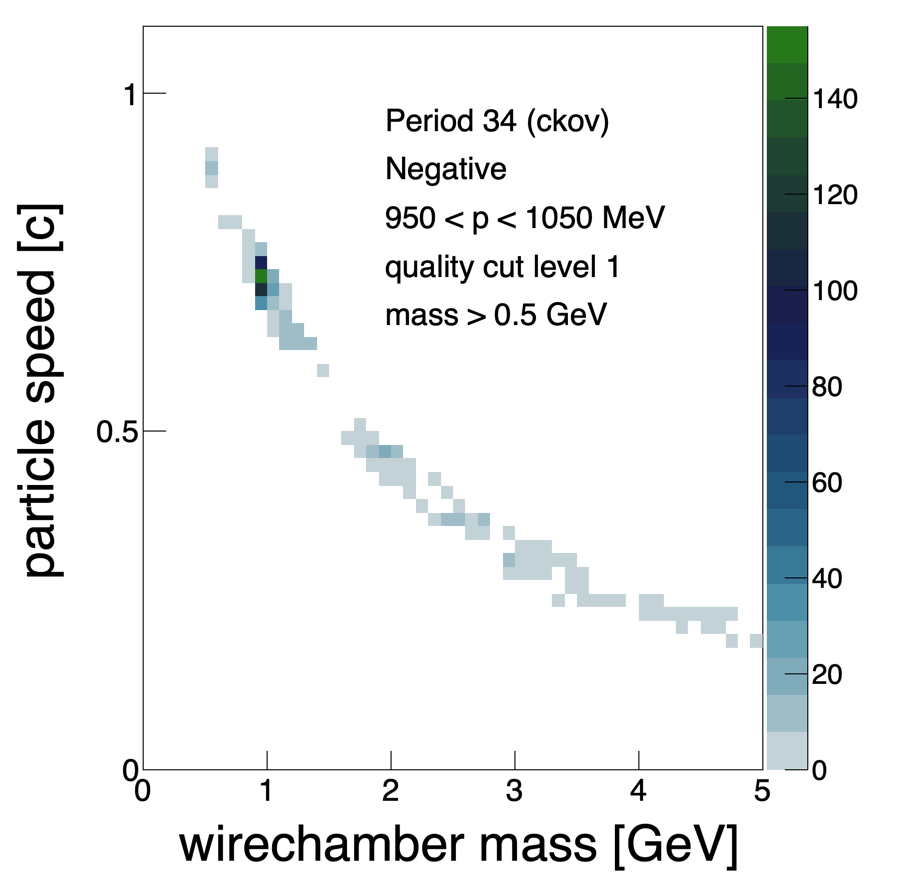
\includegraphics[width=\textwidth]{ckov_period34_mexy_level0_neg_Mom1000_Cur1_mass0.5.png}
            \caption{Mass $>$ 0.5}
            %\label{fig_mproton750}
            \end{subfigure}
             \hfill   
            \begin{subfigure}[b]{0.3\textwidth}
            \centering
            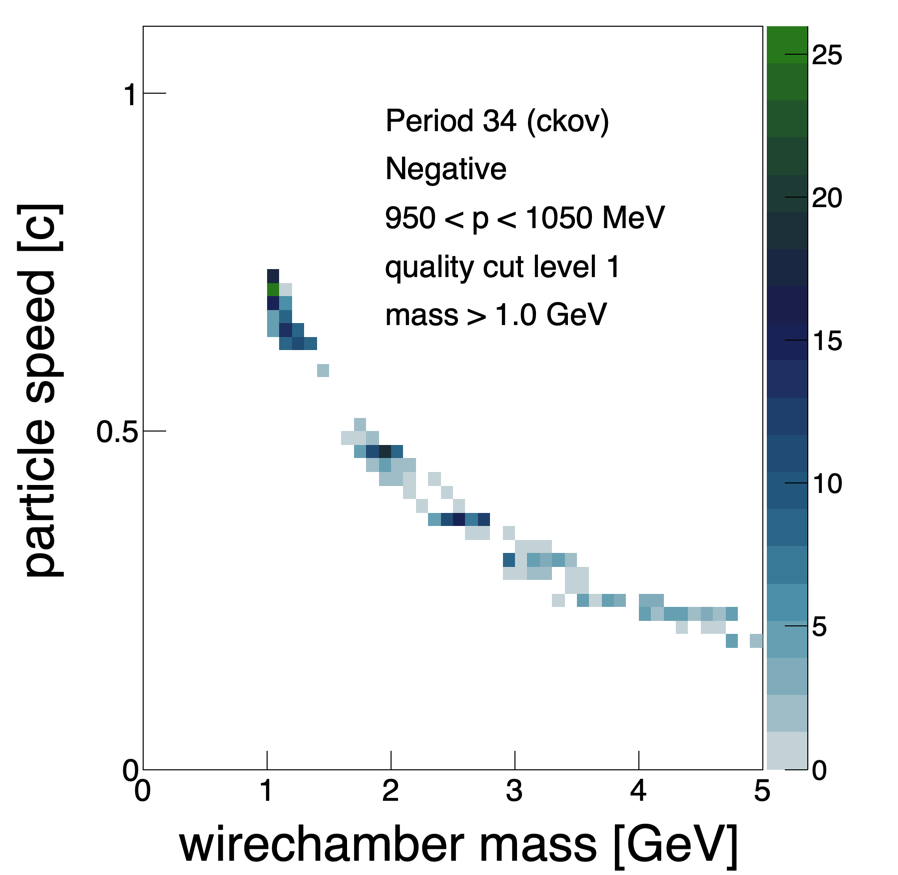
\includegraphics[width=\textwidth]{ckov_period34_mexy_level0_neg_Mom1000_Cur1_mass1.0.png}
            \caption{Mass > 1 GeV}
           % \label{fig_mproton1000}
            \end{subfigure}
            
\caption{Nicer blots }
\label{fig_beta-mass-ckov-nicer}
  \end{figure}
  
  
  
  
  
  The kaon speed distibution has two distinct peaks, which is puzzling me.  I noticed though that if I add a momentum cut to match the magnet current cut, the lower peak goes away.
  
     \begin{figure}[h]	
 \centering   
               \begin{subfigure}[b]{0.3\textwidth}
            \centering
           % 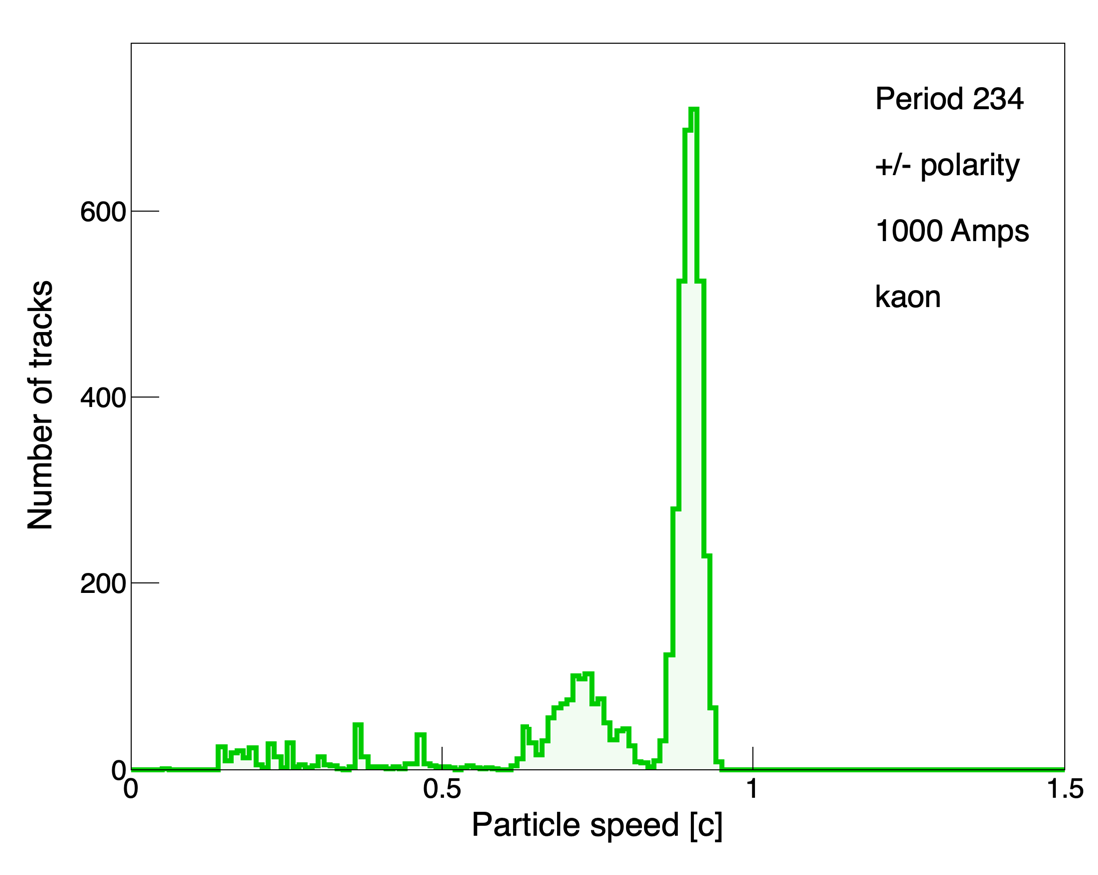
\includegraphics[width=\textwidth]{kaon-figsingle_period234_beta_level0_posneg_stats_1000Amps_nomomcut.png}
            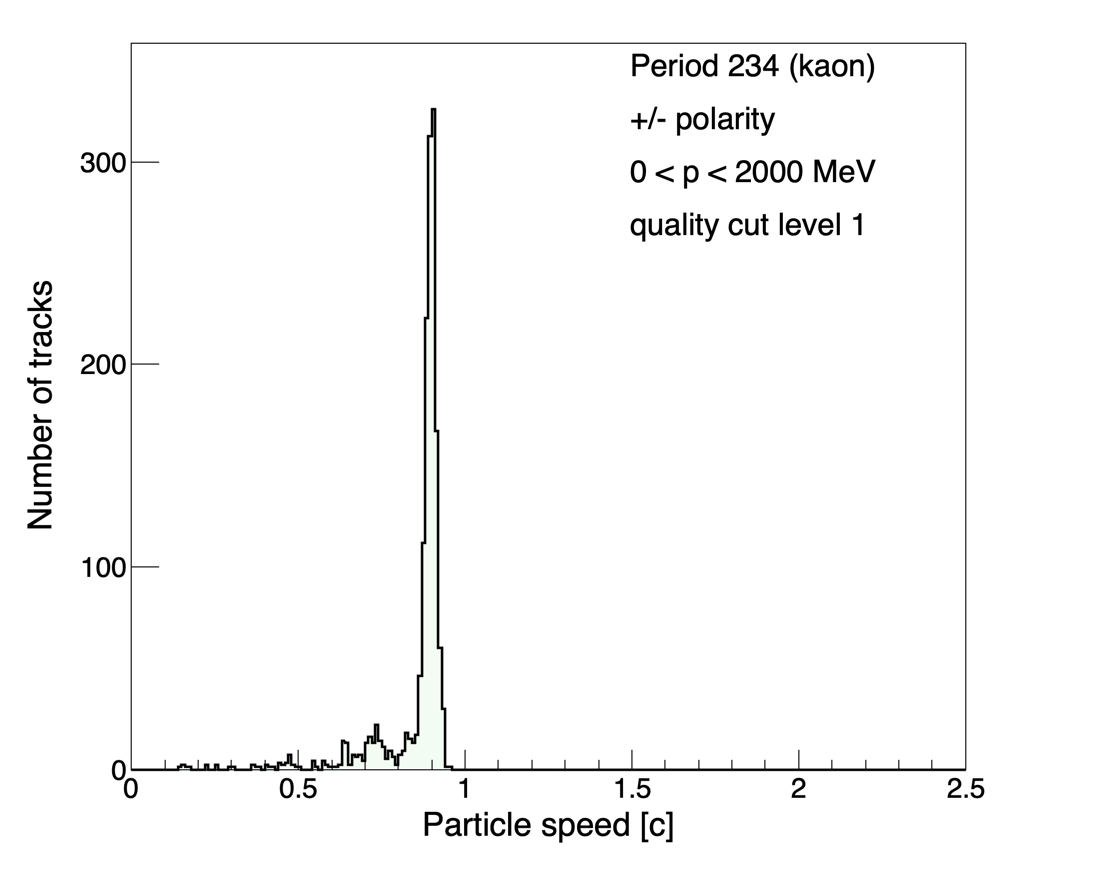
\includegraphics[width=\textwidth]{kaon_period234_beta_level0_posneg_stats_allMom_Cur1.png}
            \caption{Kaon speed}
           % \label{fig_mproton500}
            \end{subfigure}
             \hfill   
            \begin{subfigure}[b]{0.3\textwidth}
            \centering
            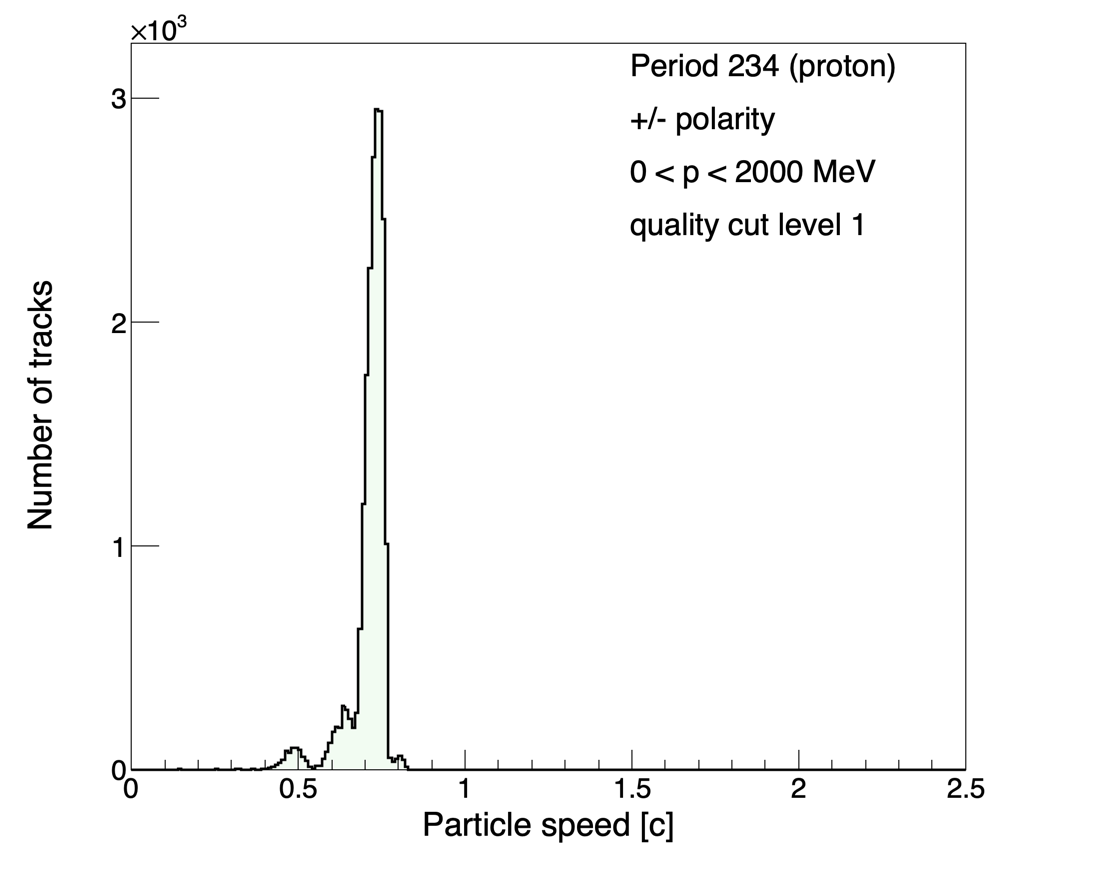
\includegraphics[width=\textwidth]{proton_period234_beta_level0_posneg_stats_allMom_Cur1.png}
            \caption{Proton speed}
            %\label{fig_mproton750}
            \end{subfigure}
             \hfill   
            \begin{subfigure}[b]{0.3\textwidth}
            \centering
            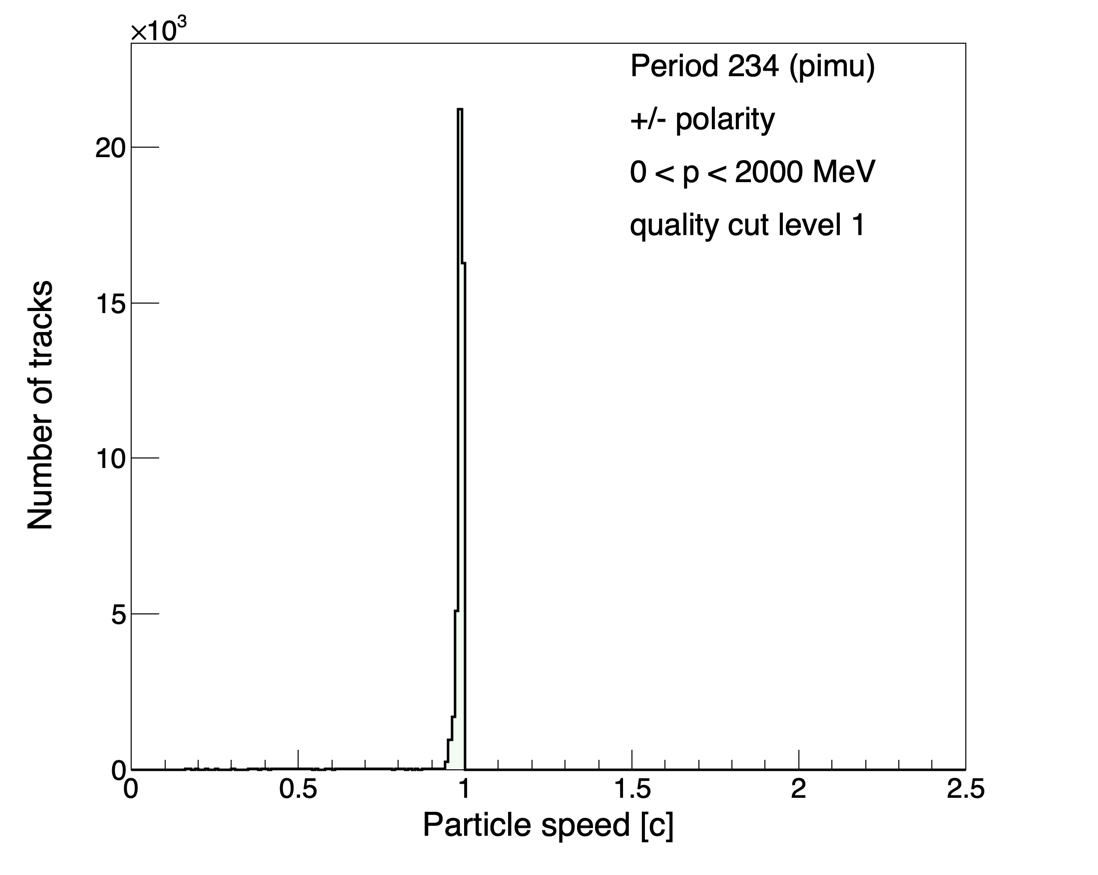
\includegraphics[width=\textwidth]{pimu_period234_beta_level0_posneg_stats_allMom_Cur1.png}
            \caption{Pion speed}
           % \label{fig_mproton1000}
            \end{subfigure}
            
                           \begin{subfigure}[b]{0.3\textwidth}
            \centering
           % 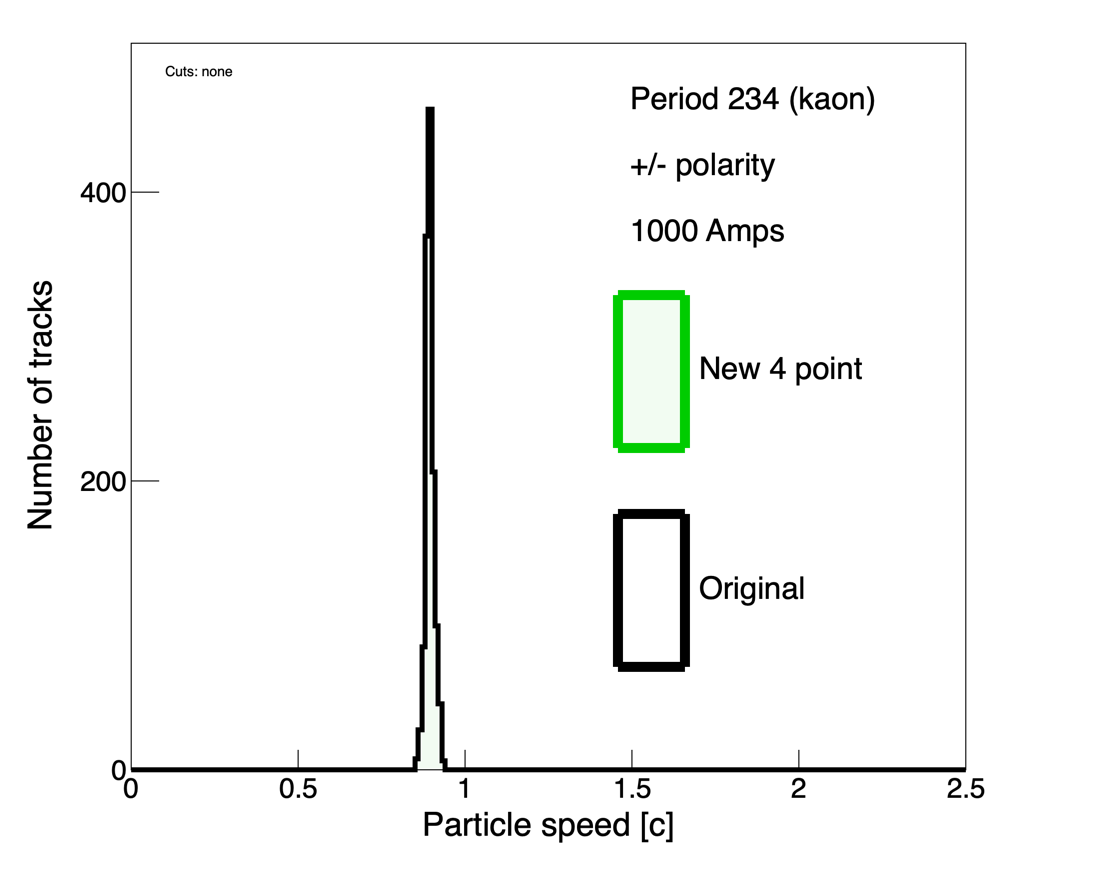
\includegraphics[width=\textwidth]{kaon-figsingle_period234_beta_level0_posneg_stats_1000Amps_momcut.png}
            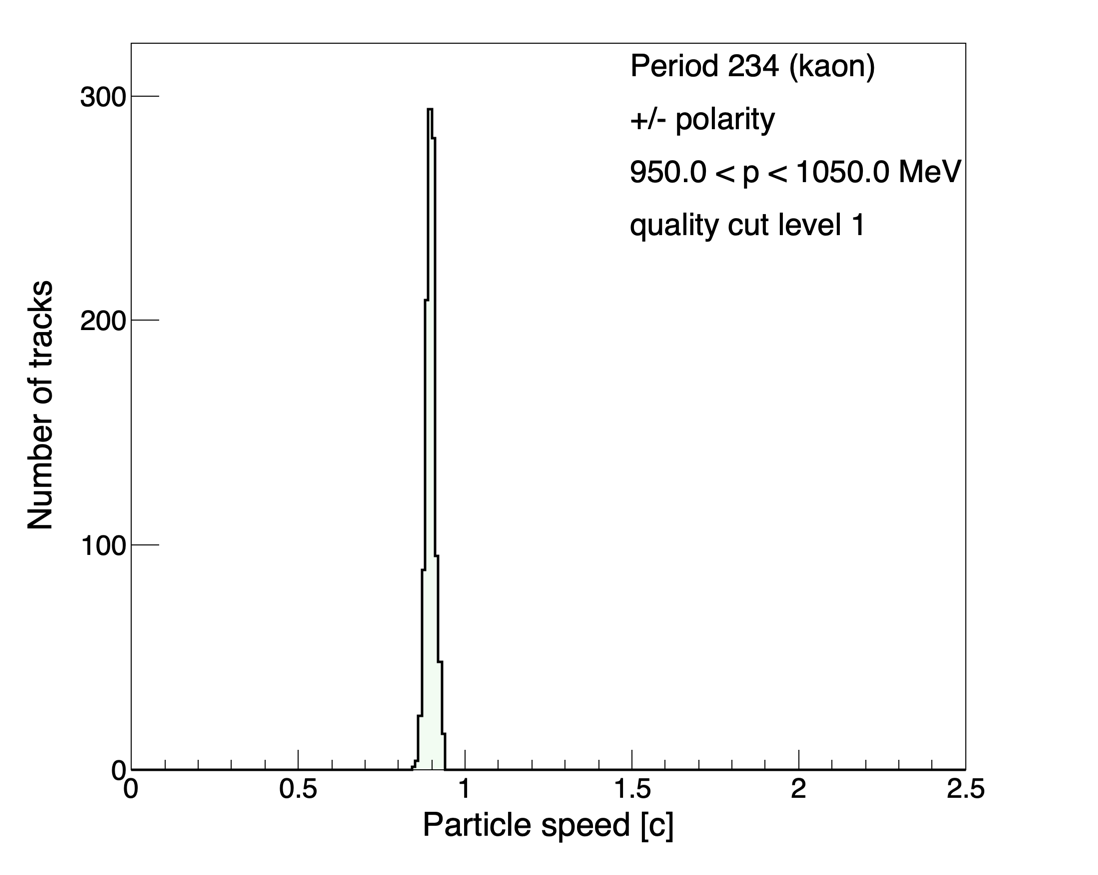
\includegraphics[width=\textwidth]{kaon_period234_beta_level0_posneg_stats_Mom1000.0_Cur1.png}
            \caption{Kaon speed}
           % \label{fig_mproton500}
            \end{subfigure}
             \hfill   
            \begin{subfigure}[b]{0.3\textwidth}
            \centering
            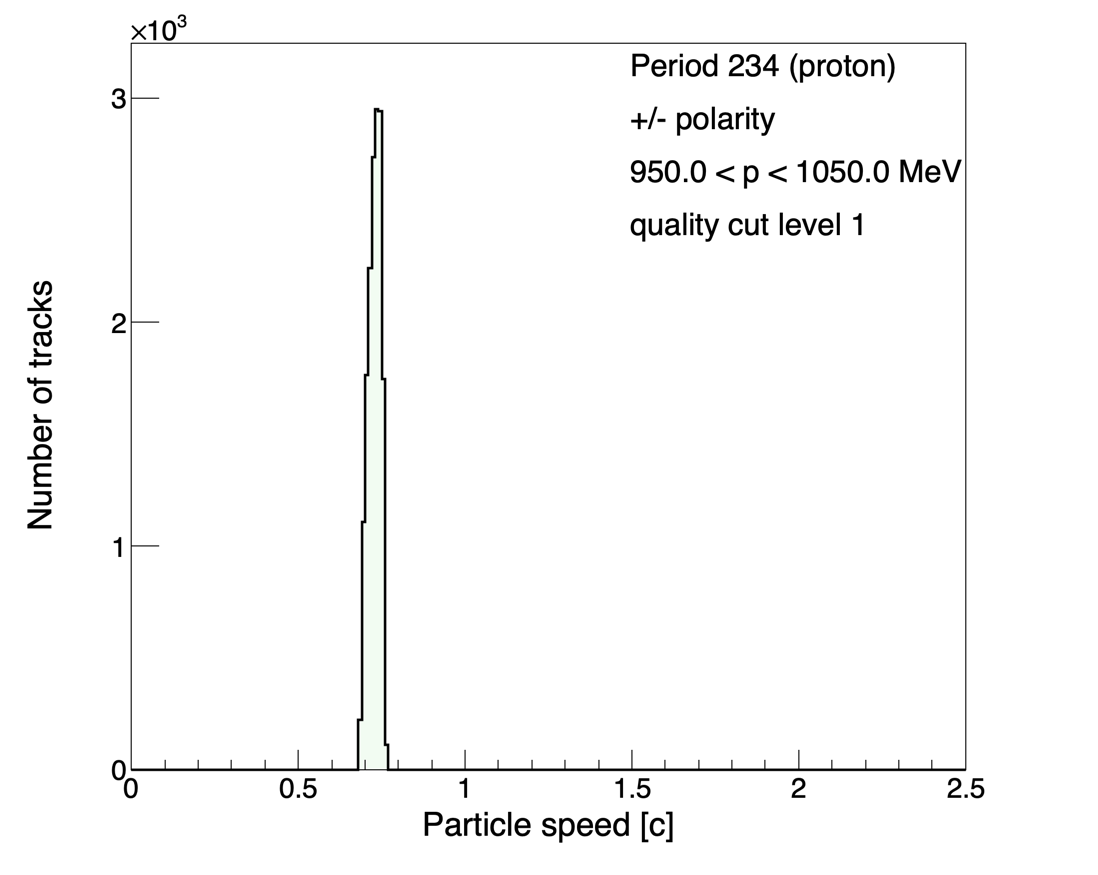
\includegraphics[width=\textwidth]{proton_period234_beta_level0_posneg_stats_Mom1000.0_Cur1.png}
            \caption{Proton speed}
            %\label{fig_mproton750}
            \end{subfigure}
             \hfill   
            \begin{subfigure}[b]{0.3\textwidth}
            \centering
            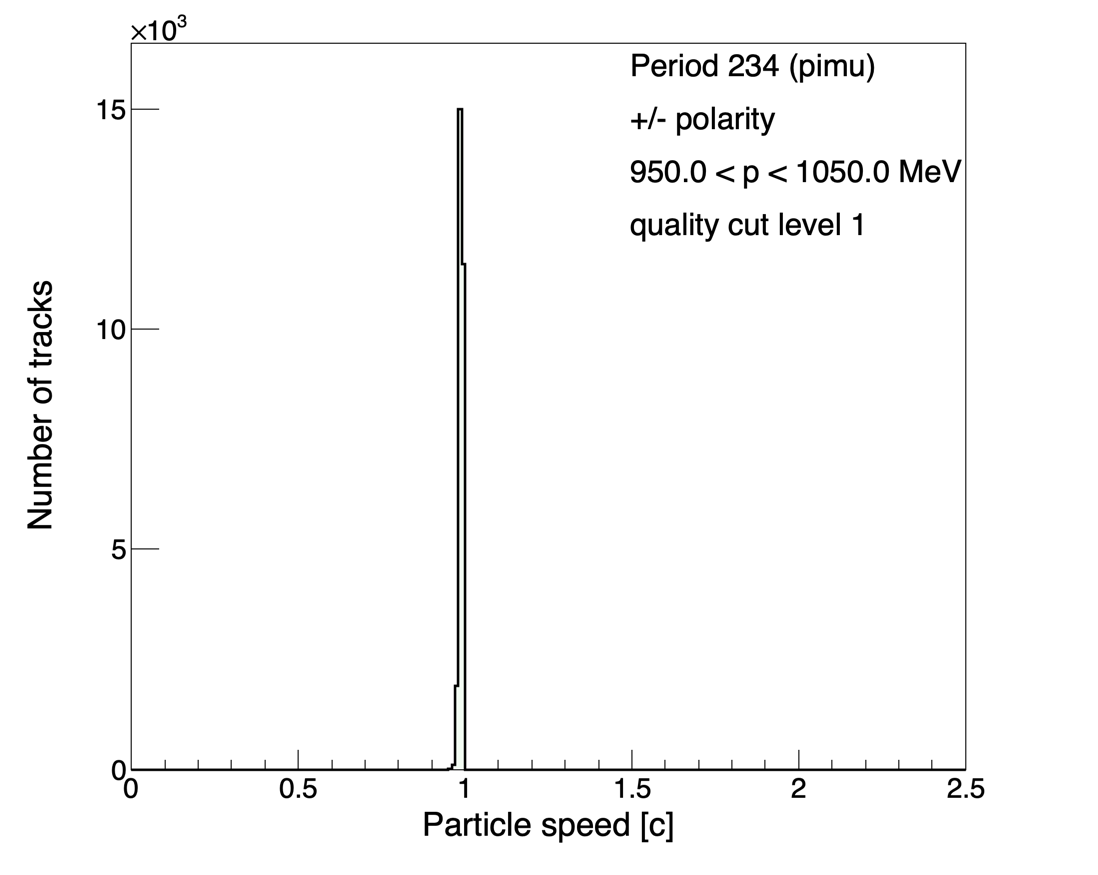
\includegraphics[width=\textwidth]{pimu_period234_beta_level0_posneg_stats_Mom1000.0_Cur1.png}
            \caption{Pion speed}
           % \label{fig_mproton1000}
            \end{subfigure}
\caption{Speed of kaons, protons, pions. Top row is without a momentum cut, bottom row is with a momentum cut consistent with the current cuts. }

  \end{figure}
  
